\part{Application des fonctions de Green à l'étude du spectre du hamiltonien}
%APPLICATION DES FONCTIONS DE GREEN A L'ETUDE DU SPECTRE DU HAMILTONTEN
% 88 
Nous avons, dans les chapitres précédents, développé le formalisme de Feynman.
Ceci nous a amené tout naturellement à l'étude de
la fonction de Green de l'équation de Schrödinger et à celle de sa transformée
de Fourier, le propagateur.

Nous avons ainsi fait connaissance avec certains objets mathématiques, d'une
utilisation très courante en physique théorique moderne et qui se révèlent très
importants pour l'étude d'un grand nombre
de problèmes.

Nous allons, dans cette partie du cours, passer en revue un
certain nombre de ces problèmes afin de nous familiariser un peu plus
avec ces objets mathématiques; ces problèmes permettent par ailleurs
d'introduire des notions très importantes qui nous serviront constamment
par la suite.

Le thème général de notre étude sera la recherche des valeurs
propres et des états propres d'un hamiltonien $\mc{H}$ constitué d'une partie
, dont le spectre est supposé connu, et d'une perturbation V. Cela pourra être
le cas d'un système libre placé dans un potentiel extérieur ou de 
deux systèmes couplés par une interaction. Nous nous attacherons, en outre,
à donner une image physique des états propres de $\mc{H}$ en étudiant comment
ils peuvent s'obtenir, dans une approche \ul{temporelle}, à partir de ceux de
$\mc{H}_0$.

Le spectre de $\mc{H}$ présentera en général deux parties : un spectre continu et un
spectre discret. Cette division sera respectée dans le
plan de cette étude qui sera le suivant :

% 89 
1°) \ul{Etude des états stationnaires de collisions} (états propres
du spectre continu) :

Nous étudierons tout d'abord, de façon mathématique, les états
propres du spectre continu (non normés) satisfaisant à certaines conditions
aux limites. Ceci nous conduira à l'équation intégrale de la diffusion, ou
équation de Lippmann-Schwinger.

Nous donnerons ensuite une image physique et temporelle de ces
états, ce qui nous conduira à la matrice S et à la théorie des collisions.
Nous terminerons par quelques méthodes d'approximation.

2°) \ul{Etude des états liés} (états propres du spectre discret) :

Nous verrons l'utilité de la résolvante pour l'étude des états
liés du hamiltonien $\mc{H}$, Ce qui nous donnera une nouvelle théorie des perturbations stationnaires.

3°) \ul{Etude des états instables} :

Nous aborderons enfin le problème des états instables qui, dans
une certaine mesure, est intermédiaire entre celui des états liés et celui
des états de collision. Nous donnerons, à partir de la résolvante une théorie de la durée de vie.

% 90
\chapter{Etats stationnaires de collision}% 6 ETATS STATIONNAIRES DE COLLISION
\section{Introduction}% A
\subsection{Description du système}% 1°) 

- Le système que nous étudierons sera celui d'une particule
dans un potentiel V($\vec{\mt{r}}$). Son hamiltonien s'écrira donc
\begin{center}
H=T+v($\vec{\mt{r}}$)
\end{center}
T représente le hamiltonien d'énergie cinétique égal à p$^2$/2m ;
V($\vec{\mt{r}}$) un potentiel décroissant avec la distance plus vite que $\frac{1}{|\vec{\mt{r}}\,|}$,
non nécessairement central.

- Nous pouvons ramener au problème précédent, celui de deux
particules A et B en interaction. Le hamiltonien s'écrit alors
\[
\mt{H} = \frac{\mt{P}_\mt{A}^2}{2\mt{m}_\mt{A}} + \frac{\mt{P}_\mt{B}^2}{2\mt{m}_\mt{B}} + \mt{V(A,B)}
\]
Le système présente l'invariance de translation et l'impulsion totale du
mouvement est donc constante.

Nous pouvons séparer le mouvement du centre de masse, rectiligne et uniforme,
du mouvement relatif dont le hamiltonien s'écrit
\begin{center}
H = T + V \hspace{2cm} avec \hspace{1cm} T = P$^2$/2m
\end{center}

\begin{minipage}[c]{.35\linewidth}
\begin{center}
en posant :
\end{center}
\end{minipage}
\hfill
\begin{minipage}[c]{.55\linewidth}
\[
\begin{array}{rl}
\mt{m} & = \frac{\mt{m}_\mt{A}\mt{m}_\mt{B}}{\mt{m}_\mt{A}+\mt{m}_\mt{B}} \hspace{1cm} \mt{(masse réduite)}\\
\vec{\mt{P}} & = \frac{\mt{m}_\mt{B}\vec{\mt{P}}_\mt{A}-\mt{m}_\mt{A}\vec{\mt{P}}_\mt{B}}{\mt{m}_\mt{A}+\mt{m}_\mt{B}}\\
\vec{\mt{r}} & =\vec{\mt{r}}_\mt{A}-\vec{\mt{r}}_\mt{B}
\end{array}
\]
\end{minipage}

Les particules A et B peuvent de plus être douées de degrés
de liberté interne (spin).

- On pourrait envisager le cas plus complexe où A et B sont
eux-mêmes des états liés de plusieurs particules, par exemple des atomes.
Le hamiltonien relatif s'écrirait alors
\[
\mc{H} = \mt{T}_\mt{A,B} + \mt{h}_\mt{A} + \mt{h}_\mt{B} + \mt{V}_\mt{AB}
\]
où T$_\mt{A,B}$ représente l'énergie cinétique relative, h$_\mt{A}$ et h$_\mt{B}$ les énergies internes des
atomes A et B, V$_\mt{AB}$ l'interaction.

Un tel cas pourrait conduire à des collisions inélastiques
(où les atomes A et B voient leur énergie interne modifiée) ou à des collisions
de réarrangement où la composition de A et B peut être elle-même
modifiée).

Nous n'étudierons pas ces cas plus complexes pour ne pas
alourdir trop l'exposé. En fait, les méthodes que nous allons étudier
s'appliquent parfaitement à ces problèmes.

Nous ne soulèverons pas non plus au début les difficultés
liées à l'indiscernabilité des particules et nous considérerons les collisions
entre deux particules différentes.

\subsection{Le spectre de T et de H}% 2°) 

\subsubsection{Spectre de T}% a)  :
C'est un spectre continu de 0 à l'infini que l'on peut écrire
E$_\mt{i}=\frac{\hbar^2\mt{k}_\mt{i}^2}{2\mt{m}}$. A chaque valeur de E$_\mt{i}$
sont associés les états propres $|\ \Phi_{\vec{\mt{k}}_\mt{i}}>$
( avec $|\ \vec{\mt{k}}_\mt{i}\ |=\mt{k}_\mt{i}$ ) qui dans la représentation $\vec{\mt{r}}$
s'écrivent $<\vec{\mt{r}}\ |\ \Phi_{\vec{\mt{k}}_\mt{i}}>=(\frac{1}{2\pi})^{3/2}\mt{ e}^{\vec{\mt{k}}_\mt{i}.\vec{\mt{r}}}$.
( Nous omettrons parfois dans la suite le facteur de normalisation $(\frac{1}{2\pi})^{3/2}$ )

 
% 92 
Le système $|\ \phi_{\vec{\mt{k}}_\mt{i}}>$, lorsqu'on a spécifié éventuellement les
états de spin des deux particules $\mu_\mt{A}$ et $\mu_\mt{B}$ constitue un système complet
de fonctions propres. (De façon rigoureuse, il faudrait écrire
$|\ \vec{\mt{k}}_\mt{i},\,\mu_\mt{A},\,\mu_\mt{B}>$.
Pour simplifier, nous écrirons les états propres $|\ \phi_{\vec{\mt{k}}_\mt{i}}>$
ou même $|\ \phi_\mt{i}>$ tant qu'il n'y aura pas d'ambiguité).

Nous ne soulèverons pas ici les difficultés liées au spectre
continu (les fonctions d'onde représentant $|\ \phi_\mt{i}>$ ne sont pas de carré
sommable et seuls les paquets d'onde ont un sens physique).

\subsubsection{Spectre de H}% b)  :
Nous allons voir qu'à chaque état propre $|\ \phi_\mt{i}>$ de T, de valeur propre
$\mt{E}_\mt{i}=\frac{\hbar^2\mt{k}_\mt{i}^2}{2\mt{m}}$, on peut associer au moins deux états propres
$|\ \psi_\mt{i}^\pm>$ du hamiltonien H, de \ul{même valeur} propre $\mt{E}_\mt{i}$

Le spectre de H comprend donc au moins une partie continue qui
va de zéro à l'infini.

On sait d'autre part que si V est attractif, il y a en plus un
spectre discret de valeurs négatives, les états correspondants étant les
états liés : le spectre de H présente donc en général l'aspect suivant :\begin{center}
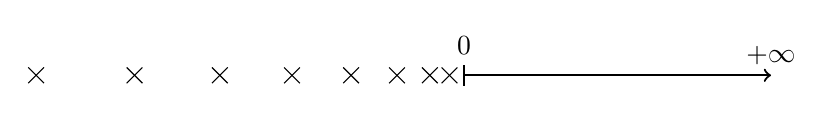
\begin{tikzpicture}
\draw [thick] (0.1,-0.13) -- (0.1,0.13) node [above]{$0$}; \draw [thick] [->] (0.1,0) -- (4,0) node [above]{$+\infty$};
\foreach \s in {1,2,...,8}
{
\draw (-\s*\s/12-0.1,0.1) -- (-\s*\s/12+0.1,-0.1);
\draw (-\s*\s/12+0.1,0.1) -- (-\s*\s/12-0.1,-0.1);
}
\end{tikzpicture} \end{center}

Notons que les $|\ \psi_\mt{i}^\pm>$, qui constituent ce qu'on appellera
les "états stationnaires de collision", ne forment donc certainement pas
en général un système complet, car ils ne représentent pas la partie
discrète du spectre.

% 93 
\subsection{Plan suivi}% 3°) 
- Nous allons tout d'abord, de façon purement mathématique, rechercher les états
propres de H ayant un comportement asymptotique donné,
que nous appellerons $|\ \psi_\mt{i}^+>$ et $|\ \psi_\mt{i}^->$ (états stationnaires de collision).
Pour cela, nous utiliserons les fonctions de Green. Nous serons conduits
à l'équation intégrale de la diffusion (\S B).

- Nous verrons ensuite à quoi correspondent physiquement les
états mathématiques ainsi introduits. Nous verrons notamment que si on
établit \ul{adiabatiquement} la perturbation V et si on appelle U l'opérateur
d'évolution correspondant à cet établissement adiabatique, alors
\[
|\ \psi_\mt{i}^+>=\lim_{\mt{t}_0\to-\infty}\mt{ U(0, t}_0\ |\ \phi_\mt{i}>
\]
\[
|\ \psi_\mt{i}^->=\lim_{\mt{t}_0\to+\infty}\mt{ U(0, t}_0\ |\ \phi_\mt{i}>
\]
ce qui justifiera les définitions d'onde entrante et d'onde sortante données à
$|\ \psi_\mt{i}^+>$ et à $|\ \psi_\mt{i}^->$

- Nous serons alors amenés à étudier la quantité 
\[
\mt{S}=\lim_{ \mt{t}_2\to-\infty,\ \mt{t}_1\to+\infty}
\mt{U}(\mt{t}_1,\mt{t}_2) \hspace{3cm} \mt{(matrice S)}
\]

- Nous verrons enfin l'utilité des états stationnaires de collision
pour le calcul des sections efficaces de collision.

\section{Approche mathématique}% B
\subsection{Problème mathématique}% 1°) 
Les états propres du spectre continu de $\mc{H}$ sont donnés par
l'équation de Schrödinger indépendante du temps :
\[
\tag{1}-\frac{\hbar^2}{2\mt{m}}\ \Delta\psi(\vec{\mt{r}}\,) + \mt{V}(\vec{\mt{r}}\,)\ \psi(\vec{\mt{r}}\,)
 = \mt{E}\ \psi(\vec{\mt{r}}\,) \hspace{3cm} (\mt{E}>0)
\]
% 94
Posons \hspace{1.5cm} E $=\frac{\hbar^2\mt{k}^2}{2\mt{m}}$ \hspace{1.5cm}
V$(\vec{\mt{r}}\,)=\frac{\hbar^2}{2\mt{m}}$ U(r) \hspace{1.5cm}
(1) devient alors
\[
\tag{2}\big[-\Delta + \mt{U}(\vec{\mt{r}}\,)\ \big]\ \psi(\vec{\mt{r}}\,)=\mt{k}^2\ \psi(\vec{\mt{r}}\,)
\]
Nous cherchons les solutions de (2) $\psi_{\vec{\mt{k}}_\mt{i}}^\pm(\vec{\mt{r}}\,)$ qui
lorsque | $\vec{\mt{r}}$ | tend vers l'infini ont pour forme asymptotique
\[
\Lambda_\pm(\vec{\mt{r}}\,)=\mt{e}^{i\vec{\mt{k}}_\mt{i}\vec{\mt{r}}}
+ \mt{f}_\pm(\vec{\mt{k}}_\mt{i},\,\theta,\,\phi)\ \frac{\mt{e}^{\pm i \mt{k}_\mt{i}\mt{r}}}{r}
\hspace{2cm} \mt{avec} \hspace{1cm} \mt{k}_\mt{i}=|\,\vec{\mt{k}}_\mt{i}\,| \ \ ;\ \ \mt{r}=|\,\vec{\mt{r}}\ |
\]

ce qui signifie que l'on a, lorsque | $\vec{\mt{r}}$ | tend vers l'infini :

\[
\tag{3}\psi_{\vec{\mt{k}}_\mt{i}}^\pm(\vec{\mt{r}}\,)-\Lambda_\pm(\vec{\mt{r}}\,)=\mt{O}\left(\frac{1}{\mt{r}}\right)
\]
Nous appellerons ces solutions ondes stationnaires de collisions entrantes
et sortantes.

Le fait qu'il existe des solutions asymptotiques de cette forme pour un
potentiel U($\vec{\mt{r}}\,$) quelconque \ul{n'est pas évident}. Nous pouvons ici
établir une condition \ul{nécessaire} de son existence : \ul{il faut que U$(\vec{\mt{r}}\,)$ décroisse plus vite que 1/r}.

En effet, aussi bien e$^{\mt{i}\vec{\mt{k}}_\mt{i}\vec{\mt{r}}}$ que
$\frac{\mt{e}^{\mt{i k}_\mt{i}\mt{r}}}{\mt{r}}$ sont solutions de
l'équation "non perturbée" $(\Delta+\mt{k}_\mt{i}^2)$ f $=$ 0.

% 95

Il en résulte que
\[
\begin{array}{rl}
\big[\Delta+\mt{k}_\mt{i}^2-\mt{U}(\vec{\mt{r}}\,)\big] \big[\mt{A}_\pm(\vec{\mt{r}}\,)-\psi_{\vec{\mt{k}}_\mt{i}}^\pm(\vec{\mt{r}}\,)\big] & = \big[\Delta+\mt{k}_\mt{i}^2-\mt{U}(\mt{r}\,)\big]\mt{A}_\pm(\vec{\mt{r}}\,) \\
 & =-\mt{U}(\vec{\mt{r}}\,)\mt{A}_\pm(\vec{\mt{r}}\,) + \frac{\mt{e}^{\pm\mt{i k}_\mt{i}\mt{r}}}{r}\ \Delta\mt{f}_\pm(\vec{\mt{k}}_\mt{i},\,\theta,\,\phi)
\end{array}
\]

Or $\Delta\mt{f}_\pm(\vec{\mt{k}}_\mt{i},\,\theta,\,\phi)$ décroit en 1/r$^2$ lorsque r $\to\infty$, quel que soit
f$_\pm(\vec{\mt{k}}_\mt{i},\,\theta,\,\phi)$ (d'après la forme du laplacien en coordonnées sphériques).
On en déduit donc (à moins que U$(\vec{\mt{r}}\,)$ décroisse plus vite que 1/r$^3$) que
la partie principale de $\big[\Delta+\mt{k}_\mt{i}^2-\mt{U}(\vec{\mt{r}}\,)\big] \big[\mt{A}_\pm(\vec{\mt{r}}\,)-\psi_{\vec{\mt{k}}_\mt{i}}^\pm(\vec{\mt{r}}\,)\big]$ est $-\mt{U}(\vec{\mt{r}}\,)\mt{e}^{i\vec{\mt{k}}_\mt{i}\vec{\mt{r}}}$.

Or, d'après la définition (3), la partie principale de
$\mt{A}_\pm(\vec{\mt{r}}\,)-\psi_{\vec{\mt{k}}_\mt{i}}^\pm(\vec{\mt{r}}\,)$
 est en 1/r$^\alpha$ avec $\alpha>1$. La partie principale de
$\big[\Delta+\mt{k}_\mt{i}^2-\mt{U}(\vec{\mt{r}}\,)\big] \big[\mt{A}_\pm(\vec{\mt{r}}\,)-\psi_{\vec{\mt{k}}_\mt{i}}^\pm(\vec{\mt{r}}\,)\big]$
doit donc également être en 1/r$^\alpha$
(à cause du terme en $\mt{k}_\mt{i}^2$, les termes en $\Delta$ et U$(\vec{\mt{r}}\,)$ conduisent à des
ordres supérieurs).

\ul{Il est donc nécessaire} que U$(\vec{\mt{r}}\,)$ décroisse en 1/r$^\alpha$ avec
$\ul{\alpha>1}$ . Nous imposerons cette condition à U$(\vec{\mt{r}}\,)$ dans la suite de cette
étude. ({\footnotesize 
Nous excluons donc le cas du potentiel coulombien en 1/r. On sait
dans ce cas traiter le problème rigoureusement (cf. Messiah, Mécanique Quantique, t. I, page 357).})

Nous montrons par le même raisonnement que $\psi_{\vec{\mt{k}}_\mt{i}}^\pm(\vec{\mt{r}}\,)$, s'il
existe, est solution de (2) avec k = k$_i$, et représente donc un état propre H d'énergie ($\hbar^2$k$_i^2$)/2m.

\subsection{Fonction de Green de $\Delta+\mt{k}_\mt{i}^2$}% 2°) 
Pour déterminer, si elles existent, les fonctions $\psi_{\vec{\mt{k}}_\mt{i}}^\pm(\vec{\mt{r}}\,)$,
solutions de (2), admettant $\mt{A}_\pm(\vec{\mt{r}}\,)$ pour forme  asymptotique, 1a méthode
de choix est celle des fonctions de Green.

% 96
Il suffit en effet d'écrire l'équation (2) formellement
sous la forme inhomogène :
\[
\tag{4}(\Delta+\mt{k}_\mt{i}^2)\ \psi(\vec{\mt{r}}\,)=\mt{U}(\vec{\mt{r}}\,)\ \psi(\vec{\mt{r}}\,)
\]
et de considérer U$(\vec{\mt{r}}\,)\ \psi(\vec{\mt{r}}\,)$ comme une "source".

Nous sommes donc amenés à chercher la fonction de Green
G$_{\vec{\mt{k}}_\mt{i}}(\vec{\mt{r}}-\vec{\mt{r}}\,')$
de l'opérateur $\Delta+\mt{k}_\mt{i}^2$ vérifiant les "bonnes conditions"
aux limites pour r$\to\infty$.

L'équation vérifiée par G$_{\vec{\mt{k}}_\mt{i}}(\vec{\mt{r}}-\vec{\mt{r}}\,')$ est
\[
\tag{5}(\Delta+\mt{k}_\mt{i}^2)\mt{G}_{\vec{\mt{k}}_\mt{i}}(\vec{\mt{r}}-\vec{\mt{r}}\,')=\delta(\vec{\mt{r}}-\vec{\mt{r}}\,')
\]

Nous ne préciserons pas à ce niveau la forme des conditions aux limites sur G.
Nous nous contenterons de choisir a priori parmi
les solutions deux fonctions G$_+$ et G$_-$ et nous vérifierons qu'elles conduisent
bien, par résolution de (4), aux fonctions $\psi_{\vec{\mt{k}}_\mt{i}}^\pm(\vec{\mt{r}}\,)$.

Pour résoudre (5), nous allons, selon une méthode qui nous
est maintenant habituelle, utiliser la transformée de Fourier : Posons
\[
\tag{6}\mt{G}_{\vec{\mt{k}}_\mt{i}}(\vec{\mt{r}}-\vec{\mt{r}}\,')=\left(\frac{1}{2\pi}\right)^3
\int \mt{G}_{\vec{\mt{k}}_\mt{i}}(\vec{\chi}\,)\mt{e}^{i\vec{\chi}(\vec{\mt{r}}-\vec{\mt{r}}\,')}\mt{d}^3\chi
\]
La transformée de Fourier de (3) conduit à :
\[
\tag{7}(-\chi^2+\mt{k}_\mt{i}^2)\ \mt{G}_{\vec{\mt{k}}_\mt{i}}(\vec{\chi})=1
\]

L'équation (7) est analogue à l'équation (27) du chapitre 5
. Sa solution générale s'écrit :
\[
\mt{G}_{\vec{\mt{k}}_\mt{i}}(\vec{\chi})=\frac{1}{2\mt{k}_\mt{i}}\left\{\mc{P}\left[\frac{1}{\chi-\mt{k}_\mt{i}}\right]-\lambda\delta(\chi-\mt{k}_\mt{i})
-\mc{P}\left[\frac{1}{\chi+\mt{k}_\mt{i}}\right]+\lambda'\delta(\chi+\mt{k}_\mt{i})\right\}
\]
Envisageons a priori les solutions
\[
\left\{
\begin{array}{rl}
\lambda & =-i\pi \\
\lambda' & =+i\pi
\end{array}
\right.
\hspace{2cm}\mt{et}\hspace{1cm}
\left\{
\begin{array}{rl}
\lambda & =+i\pi \\
\lambda' & =-i\pi
\end{array}
\right.
\]
% 97
Elles donnent
\[
\mt{G}_{\vec{\mt{k}}_\mt{i}}^\pm(\vec{\chi})=\lim_{\epsilon'\to 0_+}\frac{-1}{2\mt{k}_\mt{i}}\left[\frac{1}{\chi-\mt{k}_\mt{i}\mp\mt{i}\epsilon'}-\frac{1}{\chi+\mt{k}_\mt{i}\pm\mt{i}\epsilon'}\right]
\]
\[
=\lim_{\epsilon'\to 0_+}\frac{1}{\mt{k}_\mt{i}^2-\chi^2\pm 2\mt{i}\mt{k}_\mt{i}\epsilon'}
\]
Soit, en faisant le changement de variable $\epsilon$ = $2\mt{k}_\mt{i}\epsilon'$ :
\[
\tag{8}\mt{G}_{\vec{\mt{k}}_\mt{i}}^\pm(\vec{\chi})=\lim_{\epsilon\to 0_+}\frac{1}{\mt{k}_\mt{i}^2-\chi^2\pm \mt{i}\epsilon}
\]
Ce sont les deux fonctions G$_{\vec{\mt{k}}_\mt{i}}^\pm(\vec{\chi})$ que nous allons choisir a priori pour
notre problème : elles correspondent aux contours d'intégration des figures a) et b).

\vspace{0.3cm}
\begin{minipage}[c]{.45\linewidth}
\begin{center} 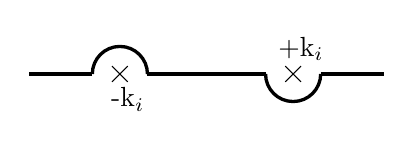
\begin{tikzpicture}
\draw [very thick] (-2.25,0) -- (-1.45,0); \draw [very thick] (-0.75,0) -- (0.75,0); \draw [very thick] (1.45,0) -- (2.25,0);
\draw (-1,-0.05) node [below]{-k$_\mt{i}$}; \draw (1.2,0.05) node [above]{+k$_\mt{i}$};
\draw (-1.2,-0.1) -- (-1,0.1); \draw (-1.2,0.1) -- (-1,-0.1); \draw [very thick] (-1.45,0)  arc (180:0:0.35);
\draw (1,-0.1) -- (1.2,0.1); \draw (1,0.1) -- (1.2,-0.1); \draw [very thick] (0.75,0)  arc (-180:0:0.35);
\end{tikzpicture}

(a) : G$_{\vec{\mt{k}}_\mt{i}}^+(\chi)$
\end{center}
\end{minipage}
\hfill
\begin{minipage}[c]{.45\linewidth}
\begin{center} 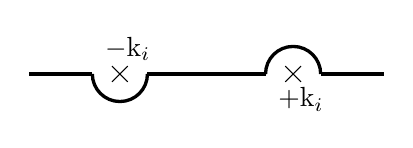
\begin{tikzpicture}
\draw [very thick] (-2.25,0) -- (-1.45,0); \draw [very thick] (-0.75,0) -- (0.75,0); \draw [very thick] (1.45,0) -- (2.25,0);
\draw (-1,0.05) node [above]{$-$k$_\mt{i}$}; \draw (1.2,-0.05) node [below]{$+$k$_\mt{i}$};
\draw (-1.2,-0.1) -- (-1,0.1); \draw (-1.2,0.1) -- (-1,-0.1); \draw [very thick] (-1.45,0)  arc (-180:0:0.35);
\draw (1,-0.1) -- (1.2,0.1); \draw (1,0.1) -- (1.2,-0.1); \draw [very thick] (0.75,0)  arc (180:0:0.35);
\end{tikzpicture}

(b) : G$_{\vec{\mt{k}}_\mt{i}}^-(\chi)$
\end{center}
\end{minipage}
\vspace{0.3cm}

Nous constatons que G$^\pm$ ne sont fonctions que de $\chi^2$ et
nous allons les écrire G$^\pm(\chi^2)$.

Pour obtenir G$_{\vec{\mt{k}}_\mt{i}}^\pm(\vec{\mt{r}}-\vec{\mt{r}'})$, il suffit d'utiliser la formule (6) : en passant en coordonnées
cylindriques avec $\vec{\mt{r}}-\vec{\mt{r}'}$ pour axe polaire et en posant $|\vec{\mt{r}}-\vec{\mt{r}'}|=\rho$, (6) devient
% 98
\[
\mt{G}_{\vec{\mt{k}}_\mt{i}}^\pm(\vec{\mt{r}}-\vec{\mt{r}}\;')=\frac{1}{(2\pi)^3}\int_0^\infty 2\pi\ \chi^2\mt{ d}\chi\mt{ G}^\pm(\chi^2)\int_0^\pi \mt{e}^{\mt{i}\chi\rho\cos\theta}\sin\theta\mt{ d}\theta
\]
et après intégration sur $\theta$ :
\[
\mt{G}_{\vec{\mt{k}}_\mt{i}}^\pm(\vec{\mt{r}}-\vec{\mt{r}}\;')=\frac{1}{\mt{i}\rho}\frac{1}{(2\pi)^2}\int_0^\infty\chi\mt{d}\chi(\mt{ e}^{\mt{i}\chi\rho}-\mt{e}^{-\mt{i}\chi\rho}) \mt{ G}^\pm(\chi^2)
\]
\[
=\frac{1}{\mt{i}\rho}\frac{1}{(2\pi)^2}\int_{-\infty}^\infty\chi\mt{d}\chi\mt{ e}^{\mt{i}\chi\rho}\mt{ G}^\pm(\chi^2)
\]
\[
=\frac{1}{\mt{i}\rho}\frac{1}{(2\pi)^2}\int_{-\infty}^\infty\chi\mt{d}\chi\mt{ e}^{\mt{i}\chi\rho}\ \frac{1}{\mt{k}_\mt{i}^2-\chi^2\pm \mt{i}\epsilon}
\]

Pour calculer cette intégrale par la méthode des résidus, il faut fermer
le contour d'intégration par un demi-grand cercle dans le plan des $\chi$ tel
que | e$^{\mt{i}\chi\rho}$ | $=$ e$^{-\mc{I}\mt{m}\chi\rho}$ tende vers zéro. Il faut donc fermer le contour
dans le demi-plan supérieur

\vspace{0.3cm}
\begin{minipage}[c]{.45\linewidth}
\begin{center} 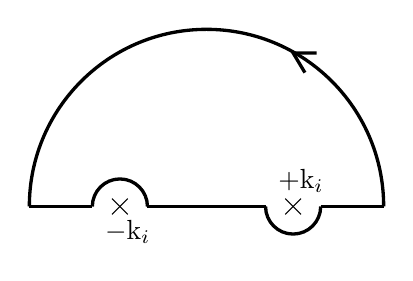
\begin{tikzpicture}
\draw [very thick] (-2.25,0) -- (-1.45,0); \draw [very thick] (-0.75,0) -- (0.75,0); \draw [very thick] (1.45,0) -- (2.25,0);
\draw (-1,-0.05) node [below]{$-$k$_\mt{i}$}; \draw (1.2,0.05) node [above]{$+$k$_\mt{i}$};
\draw (-1.2,-0.1) -- (-1,0.1); \draw (-1.2,0.1) -- (-1,-0.1); \draw [very thick] (-1.45,0)  arc (180:0:0.35);
\draw (1,-0.1) -- (1.2,0.1); \draw (1,0.1) -- (1.2,-0.1); \draw [very thick] (0.75,0)  arc (-180:0:0.35);
 \draw [very thick] (-2.25,0)  arc (180:0:2.25);
 \draw [very thick] (1.25,1.7) -- (1.1,1.95) -- (1.4,1.95);
\end{tikzpicture}

(a) : G$_{\vec{\mt{k}}_\mt{i}}^+(\chi)$
\end{center}
\end{minipage}
\hfill
\begin{minipage}[c]{.45\linewidth}
\begin{center} 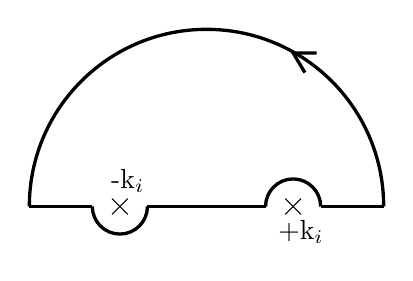
\begin{tikzpicture}
\draw [very thick] (-2.25,0) -- (-1.45,0); \draw [very thick] (-0.75,0) -- (0.75,0); \draw [very thick] (1.45,0) -- (2.25,0);
\draw (-1,0.05) node [above]{-k$_\mt{i}$}; \draw (1.2,-0.05) node [below]{+k$_\mt{i}$};
\draw (-1.2,-0.1) -- (-1,0.1); \draw (-1.2,0.1) -- (-1,-0.1); \draw [very thick] (-1.45,0)  arc (-180:0:0.35);
\draw (1,-0.1) -- (1.2,0.1); \draw (1,0.1) -- (1.2,-0.1); \draw [very thick] (0.75,0)  arc (180:0:0.35);
 \draw [very thick] (-2.25,0)  arc (180:0:2.25);
 \draw [very thick] (1.25,1.7) -- (1.1,1.95) -- (1.4,1.95);
\end{tikzpicture}

(b) : G$_{\vec{\mt{k}}_\mt{i}}^-(\chi)$
\end{center}
\end{minipage}
\vspace{0.3cm}

et on a
\[
\mt{G}_{\vec{\mt{k}}_\mt{i}}^\pm(\vec{\mt{r}}-\vec{\mt{r}}\;')=2\mt{i}\pi\times\frac{1}{\mt{i}\rho}\ \frac{1}{(2\pi)^2}\mt{Résidu}\left[\frac{\chi\mt{ e}^{\mt{i}\chi\rho}}{\mt{k}_\mt{i}^2-\chi^2\pm \mt{i}\epsilon}\right]
\]
 
Soit finalement
\[
\tag{9}\mt{G}_{\vec{\mt{k}}_\mt{i}}^\pm(\vec{\mt{r}}-\vec{\mt{r}}\;')=-\frac{1}{4\pi}\ \frac{\mt{ e}^{\pm\mt{i k}_\mt{i}|\vec{\mt{r}}-\vec{\mt{r}}\;'|}}{|\vec{\mt{r}}-\vec{\mt{r}}\;'|}
\]
G$^\pm$ sont donc les solutions à onde sortante (ou entrante)

% 99
\subsection{Equation intégrale de la diffusion}%3°) 
Reprenons maintenant l'équation (4) et traitons le second
membre U$(\vec{\mt{r}})$ $\psi(\vec{\mt{r}})$ comme une source $\rho(\vec{\mt{r}})$.

Nous savons que $\mt{G}_{\vec{\mt{k}}_\mt{i}}^\pm(\vec{\mt{r}}-\vec{\mt{r}}\;')$ permet de construire les solutions
\[
\tag{10}\psi(\vec{\mt{r}})=\int\mt{G}_{\vec{\mt{k}}_\mt{i}}^\pm(\vec{\mt{r}}-\vec{\mt{r}}\;')\ \rho(\vec{\mt{r}}\;')\mt{ d}^3\vec{\mt{r}}\;'
\]
\[
=\int\mt{G}_{\vec{\mt{k}}_\mt{i}}^\pm(\vec{\mt{r}}-\vec{\mt{r}}\;')\mt{ U}(\vec{\mt{r}}\;')\ \psi(\vec{\mt{r}}\;')\ \mt{ d}^3\vec{\mt{r}}\;'
\]

L'équation (10) est une équation intégrale qui remplace
l'équation (4) : $\psi(\vec{\mt{r}})$ satisfaisant (10), satisfait nécessairement (4).
Mais on peut ajouter à $\psi(\vec{\mt{r}})$ une solution de l'équation "sans second
membre" $(\Delta+\mt{k}_\mt{i}^2)\ \phi(\vec{\mt{r}})=0$, par exemple e$^{\mt{i}\vec{\mt{k}}_\mt{i}.\vec{\mt{r}}}$.

L'équation intégrale (10) devient alors
\[
\tag{11}\psi(\vec{\mt{r}})=\mt{e}^{\mt{i}\vec{\mt{k}}_\mt{i}.\vec{\mt{r}}}+\int\mt{G}_{\vec{\mt{k}}_\mt{i}}^\pm(\vec{\mt{r}}-\vec{\mt{r}}\;')\mt{ U}(\vec{\mt{r}}\;')\ \psi(\vec{\mt{r}}\;')\ \mt{ d}^3\vec{\mt{r}}\;'
\]

Il est facile de s'assurer que toute solution de l'équation
intégrale (11) satisfait également à l'équation (4).

Nous admettrons sans discussion que si le potentiel U$(\vec{\mt{r}})$,
qui décroît plus vite que 1/r est suffisamment régulier, l'équation intégrale (11)
admet une solution pour G$_{\vec{\mt{k}}_\mt{i}}^+(\vec{\mt{r}}-\vec{\mt{r}}\;')$ et une solution pour
G$_{\vec{\mt{k}}_\mt{i}}^-(\vec{\mt{r}}-\vec{\mt{r}}\;')$. Nous montrons par la suite que ces solutions admettent
A$_\pm(\vec{\mt{r}})$ pour forme asmptotique. Nous avons donc ramené le problème que
nous nous étions posé à la solution de l'équation intégrale :
\[
\tag{12}\psi_{\vec{\mt{k}}_\mt{i}}^\pm(\vec{\mt{r}})=\mt{e}^{\mt{i}\vec{\mt{k}}_\mt{i}.\vec{\mt{r}}}+\int\mt{G}_{\vec{\mt{k}}_\mt{i}}^\pm(\vec{\mt{r}}-\vec{\mt{r}}\;')\mt{ U}(\vec{\mt{r}}\;')\ \psi_{\vec{\mt{k}}_\mt{i}}^\pm(\vec{\mt{r}}\;')\ \mt{ d}^3\vec{\mt{r}}\;'
\]
qui porte le nom d'\ul{équation intégrale de la diffusion}.

% 100


Montrons en effet que les solutions $\psi_{\vec{\mt{k}}_\mt{i}}^\pm(\vec{\mt{r}})$ (dont nous
admettons l'existence) ont le bon comportement asymptotique.

L'intégrale de (12) convergeant, il existe nécessairement
une valeur de | $\vec{\mt{r}}$ | telle que la contribution à l'intégrale des valeurs
de $\vec{\mt{r}}\,'$ telles que | $\vec{\mt{r}}\,'$ | > | $\vec{\mt{r}}$ | soit négligeable : en d'autres termes,
on peut toujours prendre | $\vec{\mt{r}}$ | suffisamment grand pour que | $\vec{\mt{r}}\,'$ | soit
très petit devant | $\vec{\mt{r}}$ |.

On peut alors développer | $\vec{\mt{r}}-\vec{\mt{r}}\,'$ | = r-$\frac{\vec{\mt{r}}}{|\vec{\mt{r}}|}\vec{\mt{r}}\,'$
 ou encore,
en appelant $\vec{\mt{n}}$ le vecteur unitaire dans la direction $\theta$, $\phi$ de $\vec{\mt{r}}$ :
\[
|\vec{\mt{r}}-\vec{\mt{r}}\,'|=\mt{r}-\vec{\mt{n}}.\vec{\mt{r}}\,'
\]

On développe alors :
\[
\mt{G}_{\vec{\mt{k}}_\mt{i}}^\pm(\vec{\mt{r}}-\vec{\mt{r}}\;')\sim-\frac{1}{4\pi}\frac{\mt{e}^{\pm\mt{i k}_\mt{i}\mt{r}}}{\mt{r}}\times\mt{e}^{\mp\mt{i k}_\mt{i}\vec{\mt{n}}.\vec{\mt{r}}\,'}
\]
et (12) conduit à :
\[
\tag{13}\psi_{\vec{\mt{k}}_\mt{i}}^\pm(\vec{\mt{r}})\sim
\mt{e}^{\mt{i}\vec{\mt{k}}_\mt{i}.\vec{\mt{r}}}-
\frac{1}{4\pi}\frac{\mt{e}^{\mt{i k}_\mt{i}\mt{r}}}{\mt{r}}
\int\mt{e}^{\mp\mt{i k}_\mt{i}\;\vec{\mt{n}}.\vec{\mt{r}}\,'}\mt{ U}(\vec{\mt{r}}\;')
\ \psi_{\vec{\mt{k}}_\mt{i}}^\pm(\vec{\mt{r}}\;')\mt{ d}^3\vec{\mt{r}}\;'
\]
L'intégrale au second membre n'est plus qu'une fonction de k$_\mt{i}$ et de $\vec{\mt{n}}$,
c'est-à-dire de $\theta$ et $\phi$ et on peut l'écrire :
\[
\tag{14}\mt{f}_\pm(\vec{\mt{k}}_\mt{i},\theta, \phi)=
-\frac{1}{4\pi}
\int\mt{e}^{\mp\mt{i k}_\mt{i}\;\vec{\mt{n}}.\vec{\mt{r}}\,'}\mt{ U}(\vec{\mt{r}}\;')
\ \psi_{\vec{\mt{k}}_\mt{i}}^\pm(\vec{\mt{r}}\;')\mt{ d}^3\vec{\mt{r}}\;'
\]
et (13), compte tenu de (14), nous donne bien le comportement asymptotique
cherché.

Les solutions de l'équation intégrale (12) sont donc bien
les ondes stationnaires de diffusion cherchées et les fonctions de Green
choisies a priori étaient bien celles qui correspondaient au problème
étudié. De plus, la formule (14) nous donne le calcul explicite, connaissant
% 101
l'état stationnaire de collision, de la fonction f$_\pm(\vec{\mt{k}}_\mt{i},\theta, \phi)$, qui comme
nous le verrons joue un rôle essentiel dans le calcul des sections efficaces.

{\footnotesize
Nous pouvons montrer que l'intégrale (14) est toujours convergente à
l'infini si U$(\vec{\mt{r}}\,)$ décroît plus vite que 1/r. En effet nous pouvons majorer
$\psi_{\vec{\mt{k}}_\mt{i}}^\pm(\vec{\mt{r}})$ par un nombre M et U$(\vec{\mt{r}}\,')$ par 1/r'$^\alpha$ ($\alpha>1$).

En intégrant d'abord sur es angles polaires de $\vec{\mt{r}}\,'$ par rapport
à $\vec{\mt{n}}$, il vient
$
|\mt{f}|<\frac{\mt{M}}{\mt{k}_\mt{i}}\int\frac{\sin \mt{k}_\mt{i} \mt{r}'}{\mt{r}'^{\alpha+1}}\mt{ r}'^2\mt{ dr}'
$
qui converge puisque \ul{$\alpha+1>2$}.
}

Il nous reste maintenant, comme nous l'avons fait dans les
chapitres précédents, à nous affranchir de la représentation r et à donner une forme
intrinsèque à l'équation intégrale (12).

\subsection{Lien entre les fonctions de Green G$_\pm(\vec{\mt{r}}-\vec{\mt{r}}\;')$ et le
propagateur de T}%4°) 

Rappelons que le propagateur avancé ou retardé de T s'écrit
\[
\mc{G}_\pm(\mt{E}_\mt{i})=\lim_{\epsilon\to 0_+}\frac{1}{\mt{E}_\mt{i}-\mt{T}\pm\mt{i}\epsilon}=\lim_{\epsilon\to 0_+}\frac{1}{\frac{\hbar^2\mt{k}_\mt{i}^2}{2\mt{m}}-\mt{T}\pm\mt{i}\epsilon}
\]
{\footnotesize
La définition que nous donnons ici du propagateur diffère d'un terme
en i$\hbar$ de celle du chapitre V de la première partie.
}

La relation (6) peut s'écrire
\[
\tag{15}\mt{G}^\pm_{\vec{\mt{k}}_\mt{i}}(\vec{\mt{r}}-\vec{\mt{r}}\,')=\lim_{\epsilon\to 0_+}\left(\frac{1}{2\pi}\right)^3
\int
\mt{e}^{i\vec{\chi}.\vec{\mt{r}}}
\frac{1}{\mt{k}_\mt{i}^2-\chi^2\pm \mt{i}\epsilon}
\mt{e}^{-i\vec{\chi}.\vec{\mt{r}}\,'}
\mt{d}^3\vec{\chi}
\]

Appelons $|\;\vec{\chi}>$ les états propres de T de valeur propre $\frac{\hbar^2\chi^2}{2\mt{m}}$
 représentant une onde plane de vecteur d'onde $\vec{\chi}$.

% 102
Nous avons les relations
\[
\left\{
\begin{array}{rcl}
 <\vec{\mt{r}}\;|\;\vec{\chi}> & = & (\frac{1}{2\pi})^{3/2}\mt{e}^{i\vec{\chi}.\vec{\mt{r}}} \\
 <\vec{\chi}\;|\;\vec{\mt{r}}\;'> & = & (\frac{1}{2\pi})^{3/2}\mt{e}^{-i\vec{\chi}.\vec{\mt{r}}\,'}
\end{array} \right.
\]

Compte tenu de ces relations et du fait que l'ensemble des $|\;\vec{\chi}>$ est
complet, (15) peut s'écrire :
\[
\mt{G}^\pm_{\vec{\mt{k}}_\mt{i}}(\vec{\mt{r}}-\vec{\mt{r}}\,')=\frac{\hbar^2}{2\mt{m}}
\lim_{\epsilon\to 0_+}\int
<\vec{\mt{r}}\;|\;\vec{\chi}>
<\vec{\chi}\;|\;
\frac{1}{\mt{E}_\mt{i}-\mt{T}\pm\mt{i}\epsilon}
\;|\;\vec{\chi}\,'><\vec{\chi}\,'\;|\;\vec{\mt{r}}\;'>
\mt{d}^3\vec{\chi}\mt{ d}^3\vec{\chi}\,'
\]
\[=\frac{\hbar^2}{2\mt{m}}
\lim_{\epsilon\to 0_+}
<\vec{\mt{r}}\;|\;
\frac{1}{\mt{E}_\mt{i}-\mt{T}\pm\mt{i}\epsilon}
\;|\;\vec{\mt{r}}\;'>
\]
Soit
\[
\tag{16}\mt{G}^\pm_{\vec{\mt{k}}_\mt{i}}(\vec{\mt{r}}-\vec{\mt{r}}\,')=
\frac{\hbar^2}{2\mt{m}}
<\vec{\mt{r}}\;|\;
\mc{G}_\pm(\mt{E}_\mt{i})
\;|\;\vec{\mt{r}}\;'>
\]

\ul{Remarque} :
Ce résultat peut être obtenu très simplement par ailleurs : l'équation
(5) vérifiée par $\mt{G}^\pm_{\vec{\mt{k}}_\mt{i}}(\vec{\mt{r}}-\vec{\mt{r}}\,')$ est la \ul{transformée de Fourier par rapport
au temps} de l'équation vérifiée par la fonction de Green de la particule
libre (équa. 13-a, p. 6) (à un coefficient en $\hbar$ près). D'autre part les
conditions aux limites adoptées sur les "transformées de Fourier totales"
(par rapport au temps et à l'espace) sont les mêmes pour
$\mt{G}^\pm_{\vec{\mt{k}}_\mt{i}}(\vec{\mt{r}}-\vec{\mt{r}}\,')$ et
pour les fonctions de Green retardées et avancées de la particule libre
(comparer les formules (20) p. 67 et (8) de ce chapitre qui sont identiques à des
changements de variable évidents près : la "variable d'énergie"
$\hbar\omega$ est remplacée par k$_i^2$ et la "variable d'impulsion" k par $\chi$). On en déduit que
$\mt{G}^\pm_{\vec{\mt{k}}_\mt{i}}(\vec{\mt{r}}-\vec{\mt{r}}\,')$ est la \ul{transformée
de Fourier par rapport au temps}
de la fonction de Green retardée ou avancée de la particule libre (à un
coefficient en $\hbar$ près). Or nous savons (cf page 81) que la fonction de
%
Green de la particule libre est l'élément de matrice entre <$\vec{\mt{r}}$ | et | $\vec{\mt{r}}$ '>
de l'opérateur fonction de Green. $\mt{G}^\pm_{\vec{\mt{k}}_\mt{i}}(\vec{\mt{r}}-\vec{\mt{r}}\,')$ est donc l'élément de matrice entre <$\vec{\mt{r}}$ | et | $\vec{\mt{r}}$ '> de la
transfornée de Fourier (par rapport au
temps évidemment) de 1‘opérateur fonction de Green, c'est-à-dire du propagateur
avancé ou retardé (au coefficient $\hbar^2$/2m près). C'est ce qu'exprime
la formule (16) ci-dessus.

\subsection{Equation de Lippmann-Schwinger}%5°) 

Compte tenu de (16), l'équation intégrale de la diffusion (12)
peut s'écrire en considérant $\psi_{\vec{\mt{k}}_\mt{i}}^\pm(\vec{\mt{r}}\,)$ comme La fonction d'onde du vecteur
| $\psi_{\vec{\mt{k}}_\mt{i}}^\pm>$
 dans la représentation $|\;\vec{\mt{r}}>$ et en notant que
$<\vec{\mt{r}}\;'\;|$ V $\;|\;\vec{\mt{r}}\;''>=\delta$ ($\vec{\mt{r}}\;'-\vec{\mt{r}}\;'')$ V $(\vec{\mt{r}}\;'\;)$
\[
<\vec{\mt{r}}\;|\;\psi_{\vec{\mt{k}}_\mt{i}}^\pm>=
<\vec{\mt{r}}\;|\;\phi_{\vec{\mt{k}}_\mt{i}}>+
\int<\vec{\mt{r}}\;|\;\mc{G}_\pm(\mt{E}_\mt{i})\;|\;\vec{\mt{r}}\;'>
<\vec{\mt{r}}\;|\mt{ V }|\;\vec{\mt{r}}\;''><\vec{\mt{r}}\;''\;|\;\psi_{\vec{\mt{k}}_\mt{i}}^\pm>
\mt{ d}^3\vec{\mt{r}}\;'\mt{ d}^3\vec{\mt{r}}\;''
\]
ce qui représente la projection sur $|\;\vec{\mt{r}}>$ de l'équation entre vecteurs
d'états :
\[
\tag{17}|\;\psi_\mt{i}^\pm>=|\;\phi_\mt{i}>+\frac{1}{\mt{E}_\mt{i}-\mt{T}\pm\mt{i}\epsilon}
\mt{ V }|\;\psi_\mt{i}^\pm>
\]

(17) représente l'équation de Lippmann-Schwinger de la diffusion.
On peut lui associer l'équation conjuguée entre bras :
\[
\tag{18}<\psi_\mt{i}^\pm\;|=<\phi_\mt{i}\;|+
<\psi_\mt{i}^\pm\;|\mt{ V }\frac{1}{\mt{E}_\mt{i}-\mt{T}\pm\mt{i}\epsilon}
\]
dans laquelle il faut remarquer le changement de signe devant i$\epsilon$.

Nous pouvons donner à l'équation (17) une autre forme, non
intégrale. Partons de la relation générale entre opérateurs :
\[
\frac{1}{\mt{A}}-\frac{1}{\mt{B}}=\frac{1}{\mt{B}}(\mt{B}-\mt{A})\frac{1}{\mt{A}}
\]

% 104
\[
\begin{array}{rcl}
\mt{et posons \hspace{3cm} A} &=& \mt{E}_\mt{i}-\mt{T}\pm\mt{i}\epsilon\\
\mt{B} &=&\mt{E}_\mt{i}-\mt{H}\pm\mt{i}\epsilon \\
\end{array}
\]
Nous avons alors \ B$-$A$=-$V \ et
\[
\frac{1}{\mt{E}_\mt{i}-\mt{T}\pm\mt{i}\epsilon}-\frac{1}{\mt{E}_\mt{i}-\mt{H}\pm\mt{i}\epsilon}=
\frac{1}{\mt{E}_\mt{i}-\mt{H}\pm\mt{i}\epsilon}(-\mt{ V })\frac{1}{\mt{E}_\mt{i}-\mt{T}\pm\mt{i}\epsilon}
\]
Soit
\[
\frac{1}{\mt{E}_\mt{i}-\mt{T}\pm\mt{i}\epsilon}=\frac{1}{\mt{E}_\mt{i}-\mt{H}\pm\mt{i}\epsilon}
\left[1-\mt{ V }\frac{1}{\mt{E}_\mt{i}-\mt{T}\pm\mt{i}\epsilon}\right]
\]
d'où
\[
\frac{1}{\mt{E}_\mt{i}-\mt{T}\pm\mt{i}\epsilon}\mt{ V }=\frac{1}{\mt{E}_\mt{i}-\mt{H}\pm\mt{i}\epsilon}
\left[\mt{ V }-\mt{ V }\frac{1}{\mt{E}_\mt{i}-\mt{T}\pm\mt{i}\epsilon}\mt{ V }\right]
\]
\[
=\frac{1}{\mt{E}_\mt{i}-\mt{H}\pm\mt{i}\epsilon}\mt{ V }
\left[1-\frac{1}{\mt{E}_\mt{i}-\mt{T}\pm\mt{i}\epsilon}\mt{ V }\right]
\]
d'où
\[
\tag{19}\frac{1}{\mt{E}_\mt{i}-\mt{T}\pm\mt{i}\epsilon}\mt{ V }|\;\psi_\mt{i}^\pm>=
\frac{1}{\mt{E}_\mt{i}-\mt{H}\pm\mt{i}\epsilon}\mt{ V}
\left[\;|\;\psi_\mt{i}^\pm>-\frac{1}{\mt{E}_\mt{i}-\mt{T}\pm\mt{i}\epsilon}\mt{ V }|\;\psi_\mt{i}^\pm>\right]
\]
Or le terme entre crochets dans le membre de droite n'est autre que
$|\;\phi_\mt{i}>$(d'après (17)).

(17) et (19) entraînent donc
\[
\tag{20}|\;\psi_\mt{i}^\pm>=|\;\phi_\mt{i}>+\frac{1}{\mt{E}_\mt{i}-\mt{H}\pm\mt{i}\epsilon}\mt{ V }|\;\phi_\mt{i}>
\]

\ul{Remarque} :
Nous avons donc remplacé l'équation intégrale (17) par l'équation (20),
qui n'est plus intégrale. Cependant la difficulté est reportée sur le calcul des
éléments de matrice < r | $\frac{1}{\mt{E}_\mt{i}-\mt{H}\pm\mt{i}\epsilon}$ | r' > du propagateur
$\frac{1}{\mt{E}-\mt{H}\pm\mt{i}\epsilon}$ du Hamiltonien H.

% 105

Nous savons d'ailleurs (grâce à la remarque du 4°) qui se transpose sans difficulté)
que cet élément de matrice représente une des fonctions
de Green solution de l'équation :
\[
[\Delta+\mt{k}^2-\mt{U(r)}]\mt{ G}_{\vec{\mt{k}}}(\vec{\mt{r}}-\vec{\mt{r}}\,')
=\delta(\vec{\mt{r}}-\vec{\mt{r}}\,')
\]

Nous pouvons obtenir, à partir de l'équation (17), un développement en série de
l'état stationnaire de collision :
\[
\tag{21}|\;\psi_\mt{i}^\pm>=\left[1+\frac{1}{\mt{E}_\mt{i}-\mt{T}\pm\mt{i}\epsilon}\mt{ V }+\frac{1}{\mt{E}_\mt{i}-\mt{T}\pm\mt{i}\epsilon}\mt{ V }\frac{1}{\mt{E}_\mt{i}-\mt{T}\pm\mt{i}\epsilon}\mt{ V }+...\right]|\;\phi_\mt{i}>
\]

Ce développement constitue le \ul{développement de Born} de l'état stationnaire
de collision. Il nous permettra d'obtenir le déveloprement à différents
ordres de la section efficace différentielle de diffusion.

\subsection{Propriétés mathématiques des états stationnaires de collision}% 6°)
{\bf—} Etats propres de H

Nous savons déjà que les états stationnaires de collision | $\psi_\mt{i}^+>$
et | $\psi_\mt{i}^->$ sont états propres de H avec la valeur propre E$_i=\frac{\hbar^2\mt{k}_\mt{i}^2}{2\mt{m}}$.

{\bf—} Orthonormalisation

Calculons le produit scalaire $<\psi_\mt{j}^+\;|\;\psi_\mt{i}^+>$

En prenant pour $<\psi_\mt{j}^+\;|$ la forme (20) et pour $|\;\psi_\mt{i}^+>$ la forme
(17), il vient :
\[
<\psi_\mt{j}^+\;|\;\psi_\mt{i}^+>=<\phi_\mt{j}\;|\;\phi_\mt{i}>+
<\phi_\mt{j}\;|\;\frac{1}{\mt{E}_\mt{i}-\mt{T}+\mt{i}\epsilon}\mt{ V }|\;\psi_\mt{i}^+>+
<\phi_\mt{j}\;|\mt{ V }\frac{1}{\mt{E}_\mt{j}-\mt{H}-\mt{i}\epsilon}\;|\;\psi_\mt{i}^+>
\]
\[
=<\phi_\mt{j}\;|\;\phi_\mt{i}>+
\frac{1}{\mt{E}_\mt{i}-\mt{E}_\mt{j}+\mt{i}\epsilon}<\phi_\mt{j}\;|\mt{ V }|\;\psi_\mt{i}^+>+
\frac{1}{\mt{E}_\mt{j}-\mt{E}_\mt{i}-\mt{i}\epsilon}<\phi_\mt{j}\;|\mt{ V }|\;\psi_\mt{i}^+>
\]
\[
=<\phi_\mt{j}\;|\;\phi_\mt{i}>=\delta({\vec{\mt{k}}_\mt{j}}-{\vec{\mt{k}}_\mt{i}})
\]
% 106 
On montre une formule identique pour $<\psi_\mt{j}^-\;|\;\psi_\mt{i}^->$. On a donc :
\[
\tag{22}<\psi_\mt{j}^+\;|\;\psi_\mt{i}^+>=\delta({\vec{\mt{k}}_\mt{j}}-{\vec{\mt{k}}_\mt{i}})
\]
\[
\tag{23}<\psi_\mt{j}^-\;|\;\psi_\mt{i}^->=\delta({\vec{\mt{k}}_\mt{j}}-{\vec{\mt{k}}_\mt{i}})
\]
L'ensemble des $|\;\psi_\mt{i}^+>$ et l'ensemble des $|\;\psi_\mt{i}^->$, pris séparément
forment donc \ul{deux ensembles} \ul{orthonormés}.

Nous admettrons que si on ajoute à chacun de ces ensembles
les vecteurs propres $|\;\psi_\beta>$ du spectre discret de H, on obtient un système orthonormé
complet (il est évident que les $|\;\psi_\beta>$ et les $|\;\psi_\mt{i}^+>$, correspondant à des valeurs propres
différentes de H sont orthogonaux).

On a donc les relations
\[
\tag{24}\int|\;\psi_\mt{i}^+><\psi_\mt{i}^+\;|\mt{ di}+\sum_\beta|\;\psi_\beta><\psi_\beta\;|=1
\]
\[
\tag{25}\int|\;\psi_\mt{i}^-><\psi_\mt{i}^-\;|\mt{ di}+\sum_\beta|\;\psi_\beta><\psi_\beta\;|=1
\]
Calculons enfin le produit scalaire $<\psi_\mt{j}^-\;|\;\psi_\mt{i}^+>$.

Nous avons :
\[
<\psi_\mt{j}^-\;|\;\psi_\mt{i}^+>=<\phi_\mt{j}\;|\;\phi_\mt{i}>+
<\phi_\mt{j}\;|\;\frac{1}{\mt{E}_\mt{i}-\mt{T}+\mt{i}\epsilon}\mt{ V }|\;\psi_\mt{i}^+>+
<\phi_\mt{j}\;|\mt{ V }\frac{1}{\mt{E}_\mt{j}-\mt{H}+\mt{i}\epsilon}\;|\;\psi_\mt{i}^+>
\]
\[
=\delta({\vec{\mt{k}}_\mt{i}}-{\vec{\mt{k}}_\mt{j}})+<\phi_\mt{j}\;|\mt{ V }|\;\psi_\mt{i}^+>
\left\{
\frac{1}{\mt{E}_\mt{i}-\mt{E}_\mt{j}+\mt{i}\epsilon}+\frac{1}{\mt{E}_\mt{j}-\mt{E}_\mt{i}+\mt{i}\epsilon}
\right\}
\]

{\bf—} Matrice R. Matrice S.

Posons $<\phi_\mt{j}$ | V | $\psi_\mt{i}^+>=$R$_\mt{ji}$ et considérons R$_\mt{ji}$ comme l'élément de
matrice entre $<\phi_\mt{j}$ | et | $\phi_\mt{i}>$ d'une matrice R,
dite \ul{matrice de réaction}
\[
\tag{26}\mt{R}_\mt{ji}=<\phi_\mt{j}\;|\mt{ R }|\;\phi_\mt{i}>=<\phi_\mt{j}\;|\mt{ V }|\;\psi_\mt{i}^+>
\]
% 107
On a donc :
\[
<\psi_\mt{j}^-\;|\;\psi_\mt{i}^+>=\delta({\vec{\mt{k}}_\mt{i}}-{\vec{\mt{k}}_\mt{j}})+
\mt{R}_\mt{ji}
\frac{-2\mt{i}\epsilon}{\epsilon^2+(\mt{E}_\mt{i}-\mt{E}_\mt{j})^2}
\]
Or
\[
\lim_{\epsilon\to0}\frac{2\mt{i}\epsilon}{\epsilon^2+(\mt{E}_\mt{i}-\mt{E}_\mt{j})^2}=
2\mt{i}\pi\,\delta(\mt{E}_\mt{i}-\mt{E}_\mt{j})
\]
Finalement :
\[
\tag{27}<\psi_\mt{j}^-\;|\;\psi_\mt{i}^+>=\delta({\vec{\mt{k}}_\mt{i}}-{\vec{\mt{k}}_\mt{j}})-
2\mt{i}\pi\,\mt{R}_\mt{ji}\,\delta(\mt{E}_\mt{i}-\mt{E}_\mt{j})
\]
\ul{Remarque} : si E$_\mt{i}\neq\mt{E}_\mt{j}$, $|\;\psi_\mt{j}^->$ et $|\;\psi_\mt{i}^+>$
sont vecteurs propres de H correspondant
à des valeurs propres \ul{différentes}. Il est donc normal que la relation
(27) donne alors
\[
<\psi_\mt{j}^-\;|\;\psi_\mt{i}^+>=0
\]

Par définition, nous appellerons élément de matrice entre $<\phi_\mt{j}$ | et | $\phi_\mt{i}>$
\ul{de la matrice S de} \ul{collision} $<\psi_\mt{j}^-\;|\;\psi_\mt{i}^+>$, et nous
avons donc la relation :
\[
\tag{28}\mt{S}_\mt{ji}=\delta({\vec{\mt{k}}_\mt{i}}-{\vec{\mt{k}}_\mt{j}})-
2\mt{i}\pi\,\mt{R}_\mt{ji}\,\delta(\mt{E}_\mt{i}-\mt{E}_\mt{j})
\]
% 108

\section{Approche physique}% C

Nous avons, dans le \S 2, trouvé des états propres de H
ayant à l'infini un comportement asymptotique en onde plane $+$ onde sortante ou
entrante. Nous avons obtenu pour ces états une équation intégrale et un développement
en série ainsi que certaines propriétés d'orthogonalité et de fermeture.
Il nous reste maintenant à dégager la signification physique des états $|\;\psi_\mt{i}^+>$
et $|\;\psi_\mt{i}^->$.

Nous allons montrer que $|\;\psi_\mt{j}^+>$ est l'état que l'on obtient
à l'instant t $=$ 0 en étant parti de l'état libre $|\;\phi_\mt{j}>$ à l'instant
t $= -\infty$ : le couplage V transforme l'état libre initial $|\;\phi_\mt{j}>$ en $|\;\psi_\mt{j}^+>$.
De même nous allons montrer que $|\;\psi_\mt{j}^->$ est l'état à l'instant t $=$ 0, qui
sous l'effet de V deviendra l'état $|\;\phi_\mt{j}>$ à l'instant t $= +\infty$ (d'ailleurs
$|\;\psi_\mt{j}^->$ et $|\;\psi_\mt{j}^+>$ se déduisent l'un de l'autre par renversement du temps,
si l'on fait abstraction des spins).

Ces propriétés justifieront le nom d'état stationnaire
sortant ou entrant donné à $|\;\psi_\mt{j}^+>$ et à $|\;\psi_\mt{j}^->$.

\ul{Remarque importante} :
$|\;\psi_\mt{j}^\pm>$ sont des \ul{états propres} du hamiltonien H. Ils sont donc \ul{stationnaires} et
\ul{n'évoluent pas} au cours du temps. En toute rigueur, les propriétés
que nous venons d'énoncer sur les liens entre $|\;\psi_\mt{j}^\pm>$ et $|\;\phi_\mt{j}>$ sont donc
inexactes : l'état $|\;\phi_\mt{j}>$ qui n'est pas un état propre de H ne pourra pas
évoluer à l'instant t $=$ 0 vers l'état $|\;\psi_\mt{j}^+>$ et de même l'état propre
$|\;\psi_\mt{j}^->$ ne pourra pas évoluer à l'instant t $= +\infty$ vers l'état $|\;\phi_\mt{j}>$.
Cependant, nous allons voir que les propriétés que nous avons énoncées
sont des \ul{propriétés limites}, valables sous certaines conditions qu'il va
falloir préciser. Nous allons en considérer trois :

1°) Evolution du système sous l'effet d'un branchement, ou
d'une coupure, adiabatique du couplage V.

2°) Evolution d'un état initial introduit progressivement
 
% 109
3°) Evolution d'un paquet d'onde formé avec les états stationnaires de collision.

\subsection{Branchement (ou coupure) adiabatique de la perturbation}% 1°) 

\begin{center} 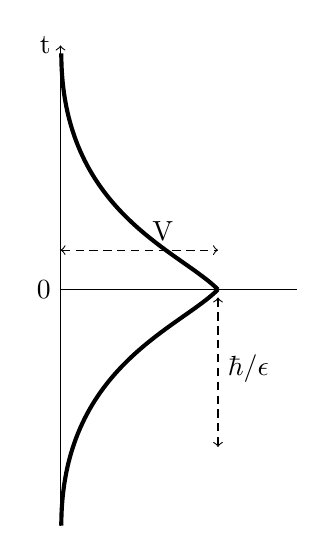
\begin{tikzpicture}
\draw (0,0) -- (3,0);
\draw [->] (0,-3) -- (0,3.1) node [left] {t};
\node at (0,0) [left]{0};
\draw [densely dashed, <->] (0,0.5)  -- (2,0.5);
\node at (1.3,0.5) [above] {V};
\draw [densely dashed, <->] (2,-0.1) -- (2,-2);
\node at (2,-1) [right]{$\hbar/\epsilon$};
\draw [line width=1.5pt] (0.01,-3) .. controls (0.01,-1) and (1.5,-0.5) .. (2,0);
\draw [line width=1.5pt] (0.01,3) .. controls (0.01,1) and (1.5,0.5) .. (2,0);
%\draw [line width=1.5pt] (1,3) .. controls (1.9,3) and (3.9,1.9) .. (4,1);
\end{tikzpicture} \end{center}

Supposons que la perturbation V stationnaire est remplacée
par une perturbation dépendant du temps
\[
\mt{V e}^{-\frac{\epsilon}{\hbar}|\mt{t}|} \hspace{2cm} \mt{(avec }\epsilon\mt{ très petit).}
\]
cela revient à considérer que la perturbation V a été branchée sur. un intervalle
de temps de l'ordre de $\hbar/\epsilon$ dans le passé et qu'elle est coupée
dans le futur avec la même constante de temps (cf figure). Lorsque $\epsilon\to 0$,
le branchement ou la coupure deviennent de plus en plus longs et la perturbation
est pratiquement égale à V sur un très grand intervalle de temps autour de t = 0 :
nous avons un branchement (ou une coupure) adiabatique de
la perturbation.

Envisageons maintenant un instant t très lointain dans le
passé et antérieur à l'établissement de la perturbation (c'est-à-dire tel
$|$t$|$ $>>\hbar/\epsilon$). Considérons qu'à cet instant, l'état initial est constitué par
une onde libre de vecteur d'onde $|\ \vec{\mt{k}}_\mt{i}>$ :
\[
|\ \psi_\mt{i}\mt{(t)}>\;=|\ \phi_\mt{i}\mt{(t)}>\;=|\ \phi_\mt{i}>\mt{e}^{-\frac{\mt{i E}_\mt{i}\mt{ t}}{\hbar}}
\]
Cherchons à déterminer l'état du système $\psi_\mt{i}\mt{(0)}>$ à l'instant t $=$ 0. Le
hamiltonien total du système est $\mc{H}$(t) $=$ T + V(t) = T $+$ V e $^{\frac{\epsilon|\mt{t}|}{\hbar}}$ et
nous pouvons développer sa fonction de Green avancée, $\mc{K}_0^+$ en fonction de
% 110
la fonction de Green avancée $\mc{K}_\epsilon^+$ de T.

On obtient alors le développement diagrammatique :
\begin{center}
\begin{tikzpicture}
\def\espace{2.3}
\draw (0,-1.5) node {$\bullet$} node [left]{t} -- (0,1.5) node {$\bullet$} node [left]{0};
\draw (\espace/2,0) node{\bf{=}};

\draw [dashed] (\espace,-1.5) node {$\bullet$} node [left]{t} -- (\espace,1.5) node {$\bullet$} node [left]{0};
\draw (3*\espace/2,0) node{\bf{+}};

\draw [dashed] (2*\espace,-1.5) node {$\bullet$} node [left]{t} -- (2*\espace+0.9,0) node {$\bullet$} ;
\draw (2*\espace+0.9,0) circle (0.25);
\draw (2*\espace+1.2,0.4) node {t'};
\draw [dashed] (2*\espace+0.9,0) -- (2*\espace,1.5) node {$\bullet$} node [left]{0};

\draw (6.5*\espace/2,0) node{\bf{+}};

\draw [dashed] (4*\espace,-1.5) node {$\bullet$} node [left]{t} -- (4*\espace+0.7,-0.5) node {$\bullet$};
\draw (4*\espace+0.7,-0.5) circle (0.25);
\draw (4*\espace+1.2,-0.4) node {t''};
\draw [dashed] (4*\espace+0.7,-0.5) -- (4*\espace-0.6,0.5) node {$\bullet$};
\draw (4*\espace-0.6,0.5) circle (0.25);
\draw (4*\espace-0.1,0.6) node {t'};
\draw [dashed] (4*\espace-0.6,0.5) -- (4*\espace,1.5) node {$\bullet$} node [left]{0};

\end{tikzpicture} \end{center}
qui permet d'écrire :
\[
\tag{29}|\ \psi_\mt{i}(0)>\;=\mc{K}_\epsilon^+(0,\mt{t})\ |\ \phi_\mt{i}(\mt{t})>
\]
\[
=\mc{K}_0^+(0,\mt{t})\ |\ \phi_\mt{i}(\mt{t})>+\frac{1}{\mt{i}\hbar}
\int\mc{K}_0^+(0,\mt{t'})\mt{ V(t') }\mc{K}_0^+(\mt{t', t})\ |\ \phi_\mt{i}(\mt{t})>\mt{ dt'}
\]
\[
+(\frac{1}{\mt{i}\hbar})^2
\int\mc{K}_0^+(0,\mt{t'})\mt{ V(t') }\mc{K}_0^+(\mt{t', t''})\ \mt{V(t'')}\ 
\mc{K}_0^+(\mt{t'', t})\ |\ \phi_\mt{i}(\mt{t})>\mt{ dt' dt''}+...
\]
avec :
\[
\tag{30}\mc{K}_0^+(\mt{t', t''})=\mt{e}^{-\mt{i}\frac{\mt{T(t'}-\mt{t''})}{\hbar}}\theta\mt{(t'}-\mt{t''})
\]
Evaluons les termes successifs du développement (29) :

\ul{1$^\mt{er}$ terme} : $|\ \phi_\mt{i}>$ étant un état propre de T, on a évidemment
\[
\mc{K}_0^+(0,\mt{t})\ |\ \phi_\mt{i}(\mt{t})>\;=|\ \phi_\mt{i}(0)>\;=|\ \phi_\mt{i}> \hspace{1.5cm} \mt{(avec les conventions de phase choisies).}
\]
% 111

\ul{2$^\mt{e}$ terme} : Le 2e terme peut s'écrire en tenant compte de (30) et de la
relation $|\ \phi_\mt{i}(\mt{t'})>\;=\mt{e}^{-\frac{\mt{i E}_\mt{i}\mt{ t'}}{\hbar}}|\ \phi_\mt{i}>$
\[
\frac{1}{\mt{i}\hbar}
\int_\mt{t}^0\mt{e}^{\frac{\mt{i T t'}}{\hbar}}\mt{e}^{-\frac{\epsilon\mt{ t'}}{\hbar}}\mt{ V }|\ \phi_\mt{i}(\mt{t'})>\mt{ dt'}=
\int_\mt{t}^0\mt{e}^{\frac{\mt{(E}_\mt{i}-\mt{T}+\mt{i}\epsilon)}{\mt{i}\hbar}}\mt{ V }|\ \phi_\mt{i}>\mt{ dt'}
\]
Comme $-$t$>>\frac{\hbar}{\epsilon}$, nous pouvons remplacer la borne inférieure par $-\infty$
et nous obtenons $\frac{1}{\mt{E}_\mt{i}-\mt{T}+\mt{i}\epsilon}\mt{ V }|\ \phi_\mt{i}>$

\ul{3$^\mt{e}$ terme} : Il s'écrit
\[
(\frac{1}{\mt{i}\hbar})^2
\int_\mt{t}^0\mt{dt'}\int_\mt{t}^\mt{t'}\mt{dt'' }
\mt{e}^{\frac{\mt{i T t'}}{\hbar}}\mt{e}^{-\frac{\epsilon\mt{ t'}}{\hbar}}
\mt{ V }\mt{e}^{-\mt{i}\frac{\mt{T(t'}-\mt{t''})}{\hbar}}\mt{e}^{-\frac{\epsilon\mt{ t''}}{\hbar}}
\mt{ V }\mt{e}^{-\frac{\mt{i E}_\mt{i}\mt{ t''}}{\hbar}}\ |\ \phi_\mt{i}>
\]
Soit, en faisant le changement de variable
\[
\left\{
\begin{array}{rcl}
\tau' & = & \mt{t'}-0 \\
\tau'' & = & \mt{t''}-\mt{t'}
\end{array}\right.
\]
\[
(\frac{1}{\mt{i}\hbar})^2
\int_\mt{t}^0\mt{d}\tau'\int_\mt{t}^0\mt{d}\tau''
\mt{ e}^{\frac{\mt{E}_\mt{i}-\mt{T}+2\mt{i}\epsilon}{\mt{i}\hbar}\tau'}
\mt{ V }\mt{e}^{\frac{\mt{E}_\mt{i}-\mt{T}+\mt{i}\epsilon}{\mt{i}\hbar}\tau''}
\mt{ V }|\ \phi_\mt{i}>
\]
Comme $-$t$>>\frac{\hbar}{\epsilon}$, nous pouvons encore remplacer la borne inférieure par $-\infty$,
et nous obtenons
\begin{center}
$\frac{1}{\mt{E}_\mt{i}-\mt{T}+2\mt{i}\epsilon}$ V 
$\frac{1}{\mt{E}_\mt{i}-\mt{T}+\mt{i}\epsilon}\mt{ V }|\ \phi_\mt{i}>$
\end{center}
etc...

La loi de formation des termes successifs devient évidente : avec les
changements de variable
\[
\left\{
\begin{array}{rcl}
\tau' & = & \mt{t'} \\
\tau'' & = & \mt{t''}-\mt{t'} \\
\tau''' & = & \mt{t'''}-\mt{t''}
\end{array}\right.
\]
etc...

% 112 
On obtient les termes
\begin{center}
$\frac{1}{\mt{E}_\mt{i}-\mt{T}+\mt{ni}\epsilon}$ V .....
$\frac{1}{\mt{E}_\mt{i}-\mt{T}+2\mt{i}\epsilon}$ V 
$\frac{1}{\mt{E}_\mt{i}-\mt{T}+\mt{i}\epsilon}\mt{ V }|\ \phi_\mt{i}>$
\end{center}
Lorsque $\epsilon\to0_+$, chaque terme de la série ainsi obtenue tend vers le terme
correspondant du développement de Born de $|\ \psi_\mt{i}^+>$.
\[
|\ \psi_\mt{i}^+>=|\ \phi_\mt{i}>
+\;\mc{G}^+(\mt{E}_\mt{i})\mt{ V }|\ \phi_\mt{i}>
+\;\mc{G}^+(\mt{E}_\mt{i})\mt{ V }\mc{G}^+(\mt{E}_\mt{i})\mt{ V }|\ \phi_\mt{i}>+\;.....
\]
Si l'on suppose que les deux développements sont uniformément convergents,
on en déduit
\[
\tag{31}\lim_{\epsilon\to0_+,\mt{t}\to-\infty} ^{|\mt{t}|>>\hbar/\epsilon}
\mc{K}^+_\epsilon(0,\mt{ t})\;|\ \phi_\mt{i}\mt{(t)}>\;=|\ \psi_\mt{i}^+>
\]
On montrerait de même que
\[
\tag{31}\lim_{\epsilon\to0_+,\mt{t}\to+\infty} ^{|\mt{t}|>>\hbar/\epsilon}
\mc{K}^-_\epsilon(0,\mt{ t})\;|\ \phi_\mt{i}\mt{(t)}>\;=|\ \psi_\mt{i}^->
\]
L'état $\mc{K}^+_\epsilon(0,\mt{ t})\ |\ \phi_\mt{i}\mt{(t)}>$ est l'état à l'instant t $=$ 0 qui a évolué à
partir d'un état initial d'onde libre établi à un instant \ul{antérieur} au
branchement adiabatique de la perturbation.

La relation (31) signifie donc qu'à la limite où le branchement
devient de plus en plus lent ($\epsilon\to0$) et où l'instant initial, tout en étant
antérieur à l'établissement de la perturbation, tend vers $-\infty$, l'onde libre
évolue vers l'état stationnaire de collision d'onde sortante. De même la
relation (32) signifie qu'à la limite où la coupure devient de plus en plus
lente ($\epsilon\to0$) et où l'instant final, tout en étant postérieur à la disparition
de la perturbation, tend vers $+\infty$, l'état stationnaire de collision
d'onde entrante évolue vers l'onde libre, Nous avons ainsi. donné une première
interprétation physique des états $|\ \psi_\mt{i}^\pm>$.
% 113
\subsection{Introduction progressive de l'état initial}% 2
Revenons au couplage stationnaire V.

Introduisons à un instant t $<$ 0 un état d'onde libre 
$|\ \phi_\mt{i}(\mt{t})>$. A l'instant t $=$ 0, cet état est devenu
\[
\tag{33}|\ \psi_\mt{i}(0)>\;=\mt{e}^{\frac{\mt{i H}}{\hbar}\mt{t}}\ |\ \phi_\mt{i}(\mt{t})>\;=
\mt{e}^{\frac{\mt{i(H}-\mt{E}_\mt{i})}{\hbar}\mt{t}}\ |\ \phi_\mt{i}(\mt{t})>
\]
$|\ \phi_\mt{i}(0)>$ ne s'exprime pas simplement car $|\ \phi_\mt{i}>$ n'est pas un état propre
de H et la relation (33), développée sur les $|\ \psi_\mt{i}^\pm>$, fait intervenir un
paquet complexe d'ondes de collision : on dit qu'on 8 un régime transitoire
dû au fait que l'état introduit n'est pas un état propre du hamiltonien.
Essayons d'échapper à cet inconvénient en envisageent un état introduit
de façon progressive entre les instants $\tau$ et 0 : de façon plus précise,
supposons qu'à l'instant t $<$ 0, on introduise un état $\phi_\mt{i}$(t), à l'instant
t$+\epsilon$ un état $\phi_\mt{i}$(t$+\epsilon$), etc. et étudions ce que devient cette
\ul{superposition linéaire} d'états, sous l'effet du hamiltonien H à l'instant t $=$ 0.
Nous obtenons un état
\[
\tag{34}|\ \psi_\mt{i}(0)>\;=\frac{1}{\tau}\int_{-\tau}^0\mt{e}^{\frac{\mt{i H}}{\hbar}\mt{t}}\ |\ \phi_\mt{i}(\mt{t})>\;\mt{dt}
\]
\[
=\frac{1}{\tau}\int_{-\tau}^0
\mt{e}^{\frac{\mt{i(H}-\mt{E}_\mt{i})}{\hbar}\mt{t}}\ |\ \phi_\mt{i}>\;\mt{dt}
\]

(le facteur 1/$\tau$ est un facteur de normalisation. Supposons en effet qu'il
n'y ait pas de couplage et que H $=$ T. Alors
$|\ \psi_\mt{i}(0)>\;=\frac{1}{\tau}\int_{-\tau}^0\mt{e}^{-\mt{i}(\mt{E}_\mt{i}-\mt{E}_\mt{i})\mt{t}}\ |\ \phi_\mt{i}>\;\mt{dt}=|\ \phi_\mt{i}>)$.

Envisageons maintenant que l'instant $\tau\to-\infty$ et introduisons alors un facteur de convergence
e$^\epsilon\mt{t}/\hbar$ qui représente un effet d'amortissement des ondes
introduites dans un passé lointain, on obtient un état
\[
\tag{35}|\ \psi_\mt{i}^{(\epsilon)}(0)>\;=\frac{\epsilon}{\hbar}\int_{-\infty}^0\mt{e}^{\frac{\mt{i H}}{\hbar}\mt{t}}
\mt{e}^{\frac{\epsilon}{\hbar}\mt{t}}\ |\ \phi_\mt{i}(\mt{t})>\;\mt{dt}
\]
\[
=\frac{\epsilon}{\hbar}\int_{-\infty}^0
\mt{e}^{\frac{\mt{i}}{\hbar}\mt{ (H}-\mt{E}_\mt{i}-\mt{i}\epsilon)\mt{ t}}\ |\ \phi_\mt{i}>\;\mt{dt}
\]
(le facteur $\epsilon/\hbar$ est encore introduit pour des raisons de normalisation :
supposons en effet que H $=$ T. Alors, on montre que $|\ \psi_\mt{i}^{\epsilon}(0)>\;=|\ \phi_\mt{i}>$).
(35) s'intègre alors immédiatement
\[
|\ \psi_\mt{i}^{(\epsilon)}(0)>\;=
\frac{\mt{i}\epsilon}{\mt{E}_\mt{i}-\mt{H}+\mt{i}\epsilon}
\ |\ \phi_\mt{i}>
\]
\[
=\frac{1}{\mt{E}_\mt{i}-\mt{H}+\mt{i}\epsilon}
\big[\mt{E}_\mt{i}-\mt{H}+\mt{i}\epsilon-(\mt{E}_\mt{i}-\mt{H})\big]
\ |\ \phi_\mt{i}>
\]
\[
=|\ \phi_\mt{i}>+
\frac{1}{\mt{E}_\mt{i}-\mt{H}+\mt{i}\epsilon}
(\mt{H}-\mt{E}_\mt{i})\ |\ \phi_\mt{i}>
\]
et finalement, puisque (H$-$E$_\mt{i}$) $|\ \phi_\mt{i}>\;=$ V $|\ \phi_\mt{i}>$ :
\[
|\ \psi_\mt{i}^{(\epsilon)}(0)>\;=
|\ \phi_\mt{i}>+
\frac{1}{\mt{E}_\mt{i}-\mt{H}+\mt{i}\epsilon}
\mt{ V }|\ \phi_\mt{i}>
\]
Ce qui n'est autre que la définition (20) de $|\ \psi_\mt{i}^+>$. D'où :
\[
\tag{36}\lim_{\epsilon\to0}\ |\ \psi_\mt{i}^{(\epsilon)}(0)>\;=|\ \psi_\mt{i}^+>
\]
Nous avons ainsi fourni une deuxième image physique de $|\ \psi_\mt{i}^+>$ :
$|\ \psi_\mt{i}^+>$ est l'état obtenu à l'instant t $=$ O à la limite où l'on a introduit
de façon progressive des états d'onde libre $|\ \phi_\mt{i}>$ depuis l'instant t $=-\infty$
avec un amortissement tendant vers zéro.

% 115

\subsection{Evolution d'un paquet d'ondes}% 3
\ul{Lemme préliminaire}

Soit f(x) une fonction suffisamment régulière de x (continue,
intégrale, différentiable) et soient g$_\pm$(t) les deux fonctions de t définies par
\[
\tag{37}\mt{g}_\pm\mt{(t)}=\lim_{\epsilon\to\,0_+}
\int_{-\infty}^{+\infty}\mt{f(x) }\frac{\mt{e}^{-\mt{ixt}}}{\mt{x}\pm\mt{i}\epsilon}\mt{ dx}
\]
Cherchons la limite de g$_\pm$(t) lorsque t$\to\pm\infty$.

\ul{Remarque} :
Il est évident que de la façon dont nous avons posé le problème, la limite
$\epsilon\to\,0_+$ , doit être prise \ul{avant} la limite t$\to\pm\infty$.
Posons f(x) $=$ f(0) $+$ f(x) $-$ f(0). Nous avons
\[
\tag{38}\mt{g}_\pm\mt{(t)}=\lim_{\epsilon\to\,0_+}\int_{-\infty}^{+\infty}
\frac{\mt{f(x)}-\mt{f(0)}}{\mt{x}\pm\mt{i}\epsilon}\mt{e}^{-\mt{ixt}}\mt{ dx}+\mt{f(0)}
\lim_{\epsilon\to\,0_+}\int_{-\infty}^{+\infty}
\frac{\mt{e}^{-\mt{ixt}}}{\mt{x}\pm\mt{i}\epsilon}\mt{ dx}
\]
La première intégrale tend vers zéro lorsque t$\to\pm\infty$.
En effet $\frac{\mt{f(x)}-\mt{f(0)}}{\mt{x}\pm\mt{i}\epsilon}$ n'a pas de singularité (pour x $=$ 0, elle tend vers f'(x) lorsque $\epsilon\to\,0$). L'intégrale sur x du produit de cette fonction régulière
par l'exponentielle oscillante e$^{-\mt{ixt}}$ dont la période en x, 1/t, tend vers
zéro lorsque t$\to\pm\infty$, tend elle-même vers zéro lorsque t$\to\pm\infty$. Si f(x) est
une courbe en "cloche" de largeur $\Delta$x, la largeur de $\frac{\mt{f(x)}-\mt{f(0)}}{\mt{x}\pm\mt{i}\epsilon}$ est du même
ordre, et on peut dire de façon plus précise que la contribution de la première
intégrale de (38) devient négligeable dès que la période 1/|t| devient petite
devant $\Delta$x, c'est-à-dire dès que |t|>>1/$\Delta$x.
Quant à la seconde intégrale
\[
\mt{f(0)}\lim_{\epsilon\to\,0_+}\int_{-\infty}^{+\infty}
\frac{\mt{e}^{-\mt{ixt}}}{\mt{x}\pm\mt{i}\epsilon}\mt{ dx}
\]
nous la calculons, selon une méthode habituelle, par les résidus en fermant
le contour vers le bas si t > 0 et vers le haut si t < 0.

% 116
Finalement, on trouve
\[
\mt{g}_+\mt{(t)}=-2\mt{i}\pi\mt{ f(0) }\theta\mt{(t)}\lim_{\epsilon\to\,0_+}
\mt{e}^{-\epsilon\mt{t}}=-2\mt{i}\pi\mt{ f(0) }\theta\mt{(t)}
\]
\[
\mt{g}_-\mt{(t)}=2\mt{i}\pi\mt{ f(0) }\theta(-\mt{t)}\lim_{\epsilon\to\,0_+}
\mt{e}^{\epsilon\mt{t}}=-2\mt{i}\pi\mt{ f(0) }\theta(-\mt{t)}
\]
Ces résultats sont indépendants de | t | et on a donc :

\[
\tag{39-a}\lim_{\mt{t}\to-\infty}\lim_{\epsilon\to\,0_+}
\int_{-\infty}^{+\infty}\mt{f(x) }
\frac{\mt{e}^{-\mt{ixt}}}{\mt{x}+\mt{i}\epsilon}\mt{ dx}=0
\]
\[
\tag{39-b}\lim_{\mt{t}\to+\infty}\lim_{\epsilon\to\,0_+}
\int_{-\infty}^{+\infty}\mt{f(x) }
\frac{\mt{e}^{-\mt{ixt}}}{\mt{x}+\mt{i}\epsilon}\mt{ dx}=-2\pi\mt{if(0)}
\]
\[
\tag{39-c}\lim_{\mt{t}\to-\infty}\lim_{\epsilon\to\,0_+}
\int_{-\infty}^{+\infty}\mt{f(x) }
\frac{\mt{e}^{-\mt{ixt}}}{\mt{x}-\mt{i}\epsilon}\mt{ dx}=2\pi\mt{if(0)}
\]
\[
\tag{39-d}\lim_{\mt{t}\to+\infty}\lim_{\epsilon\to\,0_+}
\int_{-\infty}^{+\infty}\mt{f(x) }
\frac{\mt{e}^{-\mt{ixt}}}{\mt{x}-\mt{i}\epsilon}\mt{ dx}=0
\]
Rappelons que la limite $\epsilon\to0_+$ , est prise \ul{avant} la limite |t|$\to\infty$ , cette
dernière signifiant simplement que |t|>>1/$\Delta$x, $\Delta$x étant la \mt{largeur} de f(x).
\subsubsection{Définition et propriétés du paquet d'ondes libres}% a)
Considérons, dans une situation où V est nul, un paquet \ul{d'ondes
libres} $|\ \phi\mt{(t)}>$ formé par une superposition linéaire d'ondes planes $|\ \phi_\mt{i}>$
(qui seront ici normées à l'unité) :
\[
\tag{40}|\ \phi\mt{(t)}>\;=\int\mt{c}_\mt{i}\ \mt{e}^{-\mt{i(E}_\mt{i}\mt{t)/}\hbar}\ |\ \phi_\mt{i}>\mt{di}
\]
La sommation $\int\mt{c}_\mt{i}\mt{ di}$ résume une sommation sur le module k$_\mt{i}$ et sur la
direction $\Omega_\mt{i}$ du vecteur d'onde de $|\ \phi_\mt{i}>$ :
\[
\int\mt{c}_\mt{i}\mt{ di}=\int\mt{C}(\mt{k}_\mt{i},\Omega_\mt{i})\mt{ k}_\mt{i}^2\mt{ dk}_\mt{i}\mt{ d}\Omega_\mt{i}
\]
C({k$_\mt{i},\Omega_\mt{i})$ est une fonction régulière de k$_\mt{i}$ et de $\Omega_\mt{i}$ que nous supposerons
de plus très concentrée autour des valeurs moyennes $\overline{\mt{k}_\mt{i}}$ et $\overline{\Omega_\mt{i}}$.

% 117

Nous avons ainsi défini un paquet d'ondes libres $|\ \phi\mt{(t)}>$,
dont l'évolution au cours du temps, en l'absence de V, est parfaitement
connue (équation 40).

Ce paquet d'onde possède une direction moyenne $\overline{\Omega_\mt{i}}$, une vitesse moyenne $\hbar\overline{\mt{k}_\mt{i}}/$m et une
énergie moyenne $\hbar^2\overline{\mt{k}_\mt{i}}^2/2$m. Ces résultats sont classiques.
Pour trouver la région de l'espace
où se trouve concentré le paquet d'ondes à l'instant t, il faut passer en
représentation $\vec{\mt{r}}$ et appliquer
la méthode de la phase stationnaire (cf Messiah, page 43).

Nous supposons que la phase de C({k$_\mt{i},\Omega_\mt{i})$ est telle qu'à
l'instant t = 0, le paquet $|\ \phi\mt{(t)}>$ se trouve autour de $\vec{\mt{r}} = \vec{0}$, dans la
région où sera appliqué V($\vec{\mt{r}}$).

Nous allons rappeler quelques résultats classiques relatifs
aux dimensions et à l'étalement de ce paquet d'ondes :

{\bf—} \ul{les dimensions longitudinales et transversales du paquet d'ondes} sont
d'autant plus grandes que la largeur de la fonction C({k$_\mt{i},\Omega_\mt{i})$ autour de
$\overline{\mt{k}_\mt{i}}$ et $\overline{\Omega_\mt{i}}$ est plus petite. Nous ferons l'hypothèse que les dispersions en
direction et en énergie $\Delta\Omega$ et $\Delta\mt{k}$ seront suffisamment petites pour que les
dimensions du paquet d'ondes soient très grandes devant la portée r$_0$ du
potentiel :\begin{center}
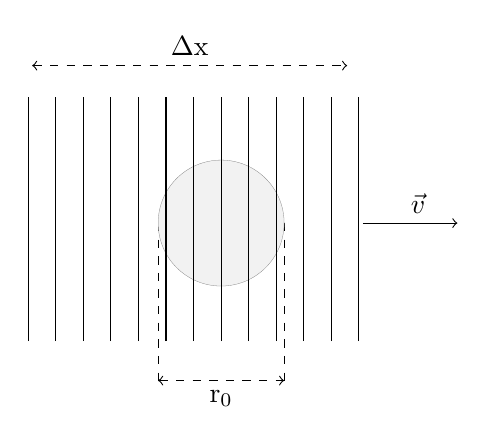
\begin{tikzpicture}
%Potentiel
\draw [dashed] (-0.8,0) -- (-0.8,-2);\draw [dashed] (0.8,0) -- (0.8,-2);
\draw [dashed, <->] (-0.8,-2) -- (0.8,-2);\draw (0,-2) node [below]{r$_0$};
\fill[color=gray!10,draw=gray, ultra thin] (0,0) circle (0.8);
%Onde
\draw [dashed, <->] (-2.4,2) -- (1.6,2);\draw (-0.4,2) node [above]{$\Delta$x};
\def\lond{0.35}
\foreach \s in {-7,-6,...,5}
{
\draw (\s*\lond,-1.5) -- (\s*\lond,1.6);
}
\draw [->] (1.8,0) -- (3,0);\draw (2.5,0) node [above]{$\vec{\mt{v}}$};
\end{tikzpicture} \end{center}
% 118

{\bf—} Etalement du paquet d'ondes : la longueur du paquet d'ondes, $\Delta$x, est
de l'ordre de 1/$\Delta$k. Le temps de passage du paquet d'ondes en un point
est $\Delta\mt{t}=\frac{\Delta\mt{x}}{\mt{v}}=\frac{\mt{m}}{\hbar\mt{k}\Delta\mt{k}}=\frac{\hbar}{\Delta\mt{E}}$,
($\Delta\mt{E}$ étant la dispersion en énergie $\frac{\hbar^2\mt{k}\Delta\mt{k}}{\mt{m}}$)
ce qui n'est autre que l'expression de la quatrième relation d'incertitude
temps-énergie.

Pendant le temps $\tau$, le paquet d'ondes subit un étalement (dû à
la dispersion des vitesses $\Delta$v$=\frac{\hbar\Delta\mt{k}}{\mt{m}}$). Cet étalement est égal à
$\tau\Delta$v$=\frac{\hbar\tau\Delta\mt{k}}{\mt{m}}$.
Cet étalement peut être considéré comme négligeable tant
qu'il est très petit devant la longueur $\Delta$x du paquet d'ondes, c'est-à-dire tant que
\[
\frac{\hbar\tau(\Delta\mt{k})^2}{\mt{m}}<<1
\]
Nous ferons l'hypothèse que pendant le temps mis par le paquet d'ondes
pour passer en un point $\Delta\mt{t}=\frac{\mt{m}}{\hbar\mt{k}\Delta\mt{k}}$, il subit un étalement négligeable,
c'est-à-dire que l'on a :
\[
\hbar\ \Delta\mt{t}\ \frac{(\Delta\mt{k})^2}{\mt{m}}<<1 \hspace{1cm} \mt{soit} \hspace{1cm} \frac{\Delta\mt{k}}{\mt{k}}<<1
\]
\ul{En résumé}, nous envisageons donc un paquet d'ondes libres $|\ \phi\mt{(t)}>$, qui
passe sur la région où règnera l‘interaction, suffisamment bien défini en
énergie et en direction pour que ses dimensions soient grandes devant la
portée effective de i'interaction V et pour que son étalement soit négligeable
durant son passage dans la région de cette portée effective.
\subsubsection{Paquet d'onde formé avec les $|\ \psi_\mt{i}^\pm>$}% b
Considérons maintenant une situation où l'interaction V($\vec{\mt{r}}$)
existe et envisageons le paquet d'ondes formé avec les états de collision
$|\ \psi_\mt{i}^+>$ (ou les états $|\ \psi_\mt{i}^->$, avec les \ul{mêmes coefficients}
C({k$_\mt{i},\Omega_\mt{i})$ que
ceux que nous avons définis pour le paquet d'ondes libres. A \ul{chaque} paquet
d'ondes libres $|\ \phi\mt{(t)}>$ vérifiant les conditions du \S précédent, nous associons
ainsi deux "paquets de collision" $|\ \psi_\mt{i}^\pm>$} définis par
\[
\tag{41}|\ \psi^\pm\mt{(t)}>\;=
\int\mt{C}_\mt{i}\ \mt{e}^{-\mt{i(E}_\mt{i}\mt{t)/}\hbar}\ |\ \psi_\mt{i}^\pm>\mt{d}_\mt{i}
\]
% 119
dont l'évolution aucours du temps est parfaitement connue (et donnée par
(41)) puisque les $|\ \psi_\mt{i}^\pm>$ sont des états propres du hamiltonien global
H $=$ T $+$ V avec la valeur propre E$_\mt{i}$.

Nous avons ainsi créé deux paquets d'ondes $|\ \psi^\pm\mt{(t)}>$ particulièrement
bien adaptés au problème de la collision. I1 nous reste à voir
le lien qui existe entre ces paquets d'ondes et le paquet d'ondes libres
$|\ \phi\mt{(t)}>$ auquel ils correspondent. Raisonnons tout d'abord sur $|\ \psi^+\mt{(t)}>$.
 
\subsubsection{Lien entre $|\ \psi^+\mt{(t)}>$ et $|\ \phi\mt{(t)}>$}% c

Remplaçons dans (41) $|\ \psi^+_\mt{i}>$ par l'expression (17) de l'équation de Lippmann-Schwinger.
On obtient :
\[
|\ \psi^+\mt{(t)}>\;=|\ \phi\mt{(t)}>+\lim_{\epsilon\to0_+}
\int\mt{d}_\mt{i}\mt{ C}_\mt{i}\ \mt{e}^{-\mt{i(E}_\mt{i}\mt{t)/}\hbar}
\ \frac{1}{\mt{E}_\mt{i}-\mt{H}+\mt{i}\epsilon}\mt{ V }|\ \psi_\mt{i}^+>
\]
Soit, en utilisant la relation de fermeture $\int\mt{d}_\mt{j}\ |\ \phi_\mt{j}><\phi_\mt{j}\ |=1$.
\[
\tag{42}
|\ \psi^+\mt{(t)}>\;=|\ \phi\mt{(t)}>+\lim_{\epsilon\to0_+}
\int\int\mt{d}_\mt{i}\mt{ d}_\mt{j}\mt{ C}_\mt{i}\ 
\ \frac{\mt{e}^{-\mt{i}\frac{\mt{E}_\mt{i}-\mt{E}_\mt{j}}{\hbar}\mt{t}}}{\mt{E}_\mt{i}-\mt{E}_\mt{j}+\mt{i}\epsilon}\mt{ R}_\mt{ji}\ |\ \phi_\mt{j}\mt{(t)}>
\]
en posant
\[
\left\{ \begin{array}{rcl}
|\ \phi_\mt{j}\mt{(t)}> & = & \mt{e}^{-\mt{i(E}_\mt{i}\mt{t)/}\hbar}\ |\ \phi_\mt{j}> \\
\mt{ R}_\mt{ji} & = & <\phi_\mt{j}\ |\ \mt{V}\ |\ \psi_\mt{i}^+> \hspace{1cm}
\mt{(selon la définition 26)}\end{array} \right.
\]
En détaillant les intégrations, (42) s'écrit :
\[
\tag{43}
|\ \psi^+\mt{(t)}>-\;|\ \phi\mt{(t)}>\;=
\int\int\mt{d}\Omega_\mt{j}\mt{ k}_\mt{j}\mt{ k}_\mt{j}^2\ |\ \phi_{\vec{\mt{k}}\,\mt{j}}\mt{(t)}>
\]
\[
\times\lim_{\epsilon\to0_+}
\int\mt{k}_\mt{i}^2\mt{ dk}_\mt{i}
\ \frac{\mt{e}^{-\mt{i}\frac{\mt{E}_\mt{i}-\mt{E}_\mt{j}}{\hbar}\mt{t}}}{\mt{E}_\mt{i}-\mt{E}_\mt{j}+\mt{i}\epsilon}
\int\mt{d}\Omega_\mt{i}\mt{ C}(\mt{k}_\mt{i }\Omega_\mt{i})
\mt{ R(k}_\mt{j}\ \Omega_\mt{j };\mt{ k}_\mt{i }\Omega_\mt{i})
\]
Nous avons posé $\mt{R}_\mt{ji}=\mt{ R(k}_\mt{j }\Omega_\mt{j };\mt{ k}_\mt{i }\Omega_\mt{i})$.
% 120
Pour simplifier cette relation, nous devons faire appel aux hypothèses
des paragraphes précédents : le coefficient C(k$_\mt{i }\Omega_\mt{i})$ n'est important qu'au voisinage
immédiat de $\Omega_\mt{i}$ (sur une étendue $\Delta\Omega$). Or R(k$_\mt{j}\ \Omega_\mt{j };\mt{ k}_\mt{i }\Omega_\mt{i})$
varie peu en $\Omega_\mt{i}$ sur $\Delta\Omega$ : à
l'approximation de Born, R(k$_\mt{j}\ \Omega_\mt{j };\mt{ k}_\mt{i }\Omega_\mt{i})$ est égal
à $<\phi_\mt{j}\ |\ \mt{V}\ |\ \phi_\mt{i}>$, transformée de Fourier du potentiel V($\vec{\mt{r}}$) à la valeur
$\vec{\mt{k}}_\mt{j}-\vec{\mt{k}}_\mt{i}$. $\vec{\mt{k}}_\mt{i}$
étant fixé, R(k$_\mt{j }\Omega_\mt{j };\mt{ k}_\mt{i }\Omega_\mt{i})$ varie donc notablement dans
l'espace des $\vec{\mt{k}}_\mt{i}$ sur des intervalles de l'ordre de 1/r$_0$, r$_0$ étant la portée
effective du potentiel V($\vec{\mt{r}}\,)$. Or au premier \S, nous avons justement choisi $\Delta\Omega$
suffisamment petit pour que l'intervalle de variation correspondant pour
$\vec{\mt{k}}_\mt{i}$ soit très petit devant 1/r$_0$. Il en résulte donc que R(k$_\mt{j}\ \Omega_\mt{j };\mt{ k}_\mt{i }\Omega_\mt{i})$
varie peu en $\Omega_\mt{i}$ sur l'intervalle $\Delta\Omega$, largeur de la fonction $\mt{C}(\mt{k}_\mt{i},\Omega_\mt{i})$. On
peut donc écrire la dernière intégration de (43) :
\[
\int\mt{d}\Omega_\mt{i}\mt{ C}(\mt{k}_\mt{i }\Omega_\mt{i})
\mt{ R(k}_\mt{j}\ \Omega_\mt{j };\mt{ k}_\mt{i }\Omega_\mt{i})\to
\mt{ R(k}_\mt{j}\ \Omega_\mt{j };\mt{ k}_\mt{i }\overline{\Omega_\mt{i}})
\int\mt{d}\Omega_\mt{i}\mt{ C}(\mt{k}_\mt{i }\Omega_\mt{i})
\]
Posons alors
\[
\tag{44}\mt{k}_\mt{i }\mt{ R(k}_\mt{j}\ \Omega_\mt{j };\mt{ k}_\mt{i }\overline{\Omega_\mt{i}})
\int\mt{d}\Omega_\mt{i}\mt{ C}(\mt{k}_\mt{i},\ \Omega_\mt{i})=\mt{ F(k}_\mt{i},\mt{ k}_\mt{j},\ \Omega_\mt{j}).
\]
La relation (3) nous conduit done à calculer
\[
\mt{ B(t},\mt{ k}_\mt{j }\Omega_\mt{j})=\lim_{\epsilon\to\;0_+}
\int\mt{k}_\mt{i}\mt{ dk}_\mt{i }\mt{ F(k}_\mt{i},\mt{ k}_\mt{j},\ \Omega_\mt{j})
\ \frac{\mt{e}^{-\mt{i}\frac{\mt{E}_\mt{i}-\mt{E}_\mt{j}}{\hbar}\mt{t}}}{\mt{E}_\mt{i}-\mt{E}_\mt{j}+\mt{i}\epsilon}
\]
c'est-à-dire, en effectuant le changement de variables E$_\mt{i}=\frac{\hbar^2\mt{k}_\mt{i}^2}{2\mt{m}}$ :
\[
\tag{45}\mt{ B(t},\mt{ k}_\mt{j }\Omega_\mt{j})=\lim_{\epsilon\to\;0_+}
\int\frac{\mt{m}}{\hbar^2}\mt{ F(E}_\mt{i},\mt{ k}_\mt{j},\ \Omega_\mt{j})
\ \frac{\mt{e}^{-\mt{i}\frac{\mt{E}_\mt{i}-\mt{E}_\mt{j}}{\hbar}\mt{t}}}{\mt{E}_\mt{i}-\mt{E}_\mt{j}+\mt{i}\epsilon}
\mt{ dE}_\mt{i }
\]
En supposant que F(E$_\mt{i},\mt{ k}_\mt{j }\Omega_\mt{j})$ est une fonction suffisamment régulière
de E$_\mt{i}$ on peut calculer $\mt{ B(t},\mt{ k}_\mt{j }\Omega_\mt{j})$ à l'aide du lemme résumé dans les
relations (39-a) et (39-b) et on a donc :
\[
\tag{46-a}\lim_{\mt{t}\to-\infty}\mt{ B(t, k}_\mt{j},\;\Omega_\mt{j})=0
\]
\[
\tag{46-b}\begin{array}{rcl}
\lim_{\mt{t}\to+\infty}\mt{ B(t, k}_\mt{j},\;\Omega_\mt{j}) & = & -\frac{2\pi\mt{i m}}{\hbar^2}\mt{ F(E}_\mt{j},\mt{ k}_\mt{j},\;\Omega_\mt{j})\\
 & = & -\frac{2\pi\mt{i m}}{\hbar^2}\mt{ k}_\mt{j}\mt{ R(k}_\mt{j}\ \Omega_\mt{j };\mt{ k}_\mt{i }\overline{\Omega_\mt{i}})
\int\mt{d}\Omega_\mt{i}\mt{ C}(\mt{k}_\mt{j }\Omega_\mt{i}) \end{array}
\]
% 121

Remarquons également que la limite |t|$\to\infty$ signifie simplement que |t|/$\hbar$
est beaucoup plus grand que l'inverse de la largeur en E$_\mt{i}$ de $\mt{ F(E}_\mt{j},\mt{ k}_\mt{j},\;\Omega_\mt{j})$
qui d'après la relation de définition (4) n'est autre que la dispersion en
énergie $\Delta$E du coefficient C(k$_\mt{i }\Omega_\mt{i})$. On peut donc remplacer la limite
|t|$\to\infty$ par la condition |t|>>$\hbar/\Delta$E, c'est-à-dire |t| grand devant
le temps de passage du paquet d'ondes libres correspondant en un point (ou
ce qui revient au même dans la région de portée du potentiel.

En résumé, (43) compte tenu des relations (46) nous conduit aux
relations
\[
\tag{47-a}\begin{array}{rcl}
\mt{ t} & \to & -\infty\\
(t &<< & -\hbar/\Delta\mt{E}) \end{array}
\hspace{2cm}|\ \psi^+\mt{(t)}>\;\sim|\ \phi\mt{(t)}>
\]
\[
\tag{47-b}\begin{array}{rcl}
\mt{ t} & \to & -\infty\\
(t &<< & -\hbar/\Delta\mt{E}) \end{array}
\hspace{2cm}|\ \psi^+\mt{(t)}>\;\sim|\ \phi\mt{(t)}>+
\int\mt{d}_\mt{j}\lambda_\mt{j}|\ \phi_\mt{j}>\mt{e}^{-i\frac{\mt{E}\mt{j}}{\hbar}\mt{t}}
\]
\ul{avec les définitions} :
\[
\tag{47-c}
\left\{ \begin{array}{rcl}
\int\mt{d}_\mt{j} & = & \int\int\mt{dk}_\mt{j}\mt{k}_\mt{j}^2\mt{d}\Omega_\mt{j}\\
\lambda_\mt{j} & = & \lambda(\mt{k}_\mt{j},\;\Omega_\mt{j}) = -\frac{2\pi\mt{i m}}{\hbar^2}\mt{ k}_\mt{j}\mt{ R(k}_\mt{j}\ \Omega_\mt{j };\mt{ k}_\mt{i }\overline{\Omega_\mt{i}})
\int\mt{d}\Omega_\mt{i}\mt{ C}(\mt{k}_\mt{j }\Omega_\mt{i})\end{array} \right.
\]
Pour le paquet d'ondes  une démonstration analogue peut être faite.
Elle conduit notamment au résultat
\[
\tag{48}\begin{array}{rcl}
\mt{ t} & \to & +\infty\\
(t & >> & -\hbar/\Delta\mt{E}) \end{array}
\hspace{2cm}|\ \psi^-\mt{(t)}>\;\sim|\ \phi\mt{(t)}>
\]
% 122
